%--%%%%%%%%%%%%%%%%%%%%%%%%%%%%%%%%%%%%
%--%%This is the LaTeX ARTICLE template for RSC journals
%--%%Copyright The Royal Society of Chemistry 2016
%--%%%%%%%%%%%%%%%%%%%%%%%%%%%%%%%%%%%%
%--%
%--%\documentclass[twoside,twocolumn,9pt]{article}
%--%\usepackage{extsizes}
%--%\usepackage[super,sort&compress,comma]{natbib} 
%--%\usepackage[version=3]{mhchem}
%--%\usepackage[left=1.5cm, right=1.5cm, top=1.785cm, bottom=2.0cm]{geometry}
%--%\usepackage{balance}
%--%\usepackage{times,mathptmx}
%--%\usepackage{sectsty}
%--%\usepackage{graphicx} 
%--%\usepackage{lastpage}
%--%\usepackage[format=plain,justification=justified,singlelinecheck=false,font={stretch=1.125,small,sf},labelfont=bf,labelsep=space]{caption}
%--%\usepackage{float}
%--%\usepackage{fancyhdr}
%--%\usepackage{color}
%--%\usepackage{fnpos}
%--%\usepackage[english]{babel}
%--%\usepackage{array}
%--%\usepackage{droidsans}
%--%\usepackage{charter}
%--%\usepackage[T1]{fontenc}
%--%\usepackage[usenames,dvipsnames]{xcolor}
%--%\usepackage{setspace}
%--%\usepackage[compact]{titlesec}
%--%%%%Please don't disable any packages in the preamble, as this may cause the template to display incorrectly.%%%
%--%
%--%%\usepackage{epstopdf}%This line makes .eps figures into .pdf - please comment out if not required.
%--%
%--%%%%%
%--%\usepackage[utf8]{inputenc}
%--%\usepackage{subfigure}
%--%\usepackage{amsfonts}
%--%\usepackage{amsgen}
%--%\usepackage{amsbsy}
%--%\usepackage{amsmath}
%--%\usepackage{amssymb}
%--%\usepackage{mathrsfs}
%--%\usepackage{mathtools}
%--%\usepackage{bm}
%--%\usepackage{epstopdf}
%--%\usepackage{caption}
%--%\usepackage{tabularx}
%--%\usepackage{tabu}
%--%\usepackage{xcolor}
%--%\usepackage{nicefrac}
%--%\usepackage{enumitem}
%--%\usepackage[ruled]{algorithm2e}
%--%\usepackage{url}
%--%
%--%\newcommand{\xx}[1]{\textcolor{black}{#1}}
%--%\newcommand\etal{\textit{et al.\ }}
%--%\newcommand\viz{\textit{viz. }}
%--%\newcommand{\e}[1]{\ensuremath{\times 10^{#1}}}
%--%\newcommand\etc{\textit{etc}}
%--%\DeclarePairedDelimiter\abs{\lvert}{\rvert}
%--%
%--%%\bibliographystyle{unsrt}  % references listed in order of appearance
%--%
%--%\definecolor{cream}{RGB}{222,217,201}
%--%
%--%
%--%
%--%\begin{document}
%--%
%--%\pagestyle{fancy}
%--%\thispagestyle{plain}
%--%\fancypagestyle{plain}{
%--%
%--%%%%HEADER%%%
%--%\fancyhead[C]{\includegraphics[width=18.5cm]{head_foot/header_bar}}
%--%\fancyhead[L]{\hspace{0cm}\vspace{1.5cm}\includegraphics[height=30pt]{head_foot/SM}}
%--%\fancyhead[R]{\hspace{0cm}\vspace{1.7cm}\includegraphics[height=55pt]{head_foot/RSC_LOGO_CMYK}}
%--%\renewcommand{\headrulewidth}{0pt}
%--%}
%--%%%%END OF HEADER%%%
%--%
%--%%%%PAGE SETUP - Please do not change any commands within this section%%%
%--%\makeFNbottom
%--%\makeatletter
%--%\renewcommand\LARGE{\@setfontsize\LARGE{15pt}{17}}
%--%\renewcommand\Large{\@setfontsize\Large{12pt}{14}}
%--%\renewcommand\large{\@setfontsize\large{10pt}{12}}
%--%\renewcommand\footnotesize{\@setfontsize\footnotesize{7pt}{10}}
%--%\makeatother
%--%
%--%\renewcommand{\thefootnote}{\fnsymbol{footnote}}
%--%\renewcommand\footnoterule{\vspace*{1pt}% 
%--%\color{cream}\hrule width 3.5in height 0.4pt \color{black}\vspace*{5pt}} 
%--%\setcounter{secnumdepth}{5}
%--%
%--%\makeatletter 
%--%\renewcommand\@biblabel[1]{#1}            
%--%\renewcommand\@makefntext[1]% 
%--%{\noindent\makebox[0pt][r]{\@thefnmark\,}#1}
%--%\makeatother 
%--%\renewcommand{\figurename}{\small{Fig.}~}
%--%\sectionfont{\sffamily\Large}
%--%\subsectionfont{\normalsize}
%--%\subsubsectionfont{\bf}
%--%\setstretch{1.125} %In particular, please do not alter this line.
%--%\setlength{\skip\footins}{0.8cm}
%--%\setlength{\footnotesep}{0.25cm}
%--%\setlength{\jot}{10pt}
%--%\titlespacing*{\section}{0pt}{4pt}{4pt}
%--%\titlespacing*{\subsection}{0pt}{15pt}{1pt}
%--%%%%END OF PAGE SETUP%%%
%--%
%--%%%%FOOTER%%%
%--%\fancyfoot{}
%--%\fancyfoot[LO,RE]{\vspace{-7.1pt}\includegraphics[height=9pt]{head_foot/LF}}
%--%\fancyfoot[CO]{\vspace{-7.1pt}\hspace{13.2cm}\includegraphics{head_foot/RF}}
%--%\fancyfoot[CE]{\vspace{-7.2pt}\hspace{-14.2cm}\includegraphics{head_foot/RF}}
%--%\fancyfoot[RO]{\footnotesize{\sffamily{1--\pageref{LastPage} ~\textbar  \hspace{2pt}\thepage}}}
%--%\fancyfoot[LE]{\footnotesize{\sffamily{\thepage~\textbar\hspace{3.45cm} 1--\pageref{LastPage}}}}
%--%\fancyhead{}
%--%\renewcommand{\headrulewidth}{0pt} 
%--%\renewcommand{\footrulewidth}{0pt}
%--%\setlength{\arrayrulewidth}{1pt}
%--%\setlength{\columnsep}{6.5mm}
%--%\setlength\bibsep{1pt}
%--%%%%END OF FOOTER%%%
%--%
%--%%%%FIGURE SETUP - please do not change any commands within this section%%%
%--%\makeatletter 
%--%\newlength{\figrulesep} 
%--%\setlength{\figrulesep}{0.5\textfloatsep} 
%--%
%--%\newcommand{\topfigrule}{\vspace*{-1pt}% 
%--%\noindent{\color{cream}\rule[-\figrulesep]{\columnwidth}{1.5pt}} }
%--%
%--%\newcommand{\botfigrule}{\vspace*{-2pt}% 
%--%\noindent{\color{cream}\rule[\figrulesep]{\columnwidth}{1.5pt}} }
%--%
%--%\newcommand{\dblfigrule}{\vspace*{-1pt}% 
%--%\noindent{\color{cream}\rule[-\figrulesep]{\textwidth}{1.5pt}} }
%--%
%--%\makeatother
%--%%%%END OF FIGURE SETUP%%%
%--%
%--%%%%TITLE, AUTHORS AND ABSTRACT%%%
%--%\twocolumn[
%--%  \begin{@twocolumnfalse}
%--%\vspace{3cm}
%--%\sffamily
%--%\begin{tabular}{m{4.5cm} p{13.5cm} }
%--%
%--%\includegraphics{head_foot/DOI} & \noindent\LARGE{\textbf{Flow-assisted droplet assembly in a 3D microfluidic channel$^\dag$}} \\%Article title goes here instead of the text "This is the title"
%--%\vspace{0.3cm} & \vspace{0.3cm} \\
%--%
%--% & \noindent\large{Zhouyang Ge,$^{\ast}$ Outi Tammisola, and Luca Brandt} \\%Author names go here instead of "Full name", etc.
%--%
%--%\includegraphics{head_foot/dates} & \noindent\normalsize{%The abstract should be a single paragraph which summarises the content of the article. Any references in the abstract should be written out in full \textit{e.g.}\ [Surname \textit{et al., Journal Title}, 2000, \textbf{35}, 3523].
%--%Self-assembly of soft matter, such as droplets or colloids, has become a promising scheme to engineer novel materials, model living matter, and explore non-equilibrium statistical mechanics. In this article, we present detailed numerical simulations of few non-Brownian droplets in various flow conditions, specifically, focusing on their self-assembly within a short distance in a three-dimensional ($3D$) microfluidic channel, cf.\ [Shen \textit{et al., Adv. Sci.}, 2016, \textbf{3}(6):1600012]. Contrary to quasi two-dimensional ($q2D$) systems, where dipolar interaction is the key mechanism for droplet rearrangement, droplets in $3D$ confinement produce much less disturbance to the underlying flow, thus experiencing weaker dipolar interactions. Using confined simple shear and Poiseuille flows as reference flows, we show that the droplet dynamics is mostly affected by the shear-induced cross-stream migration, which favors chain structures if the droplets are under an attractive depletion force. For more compact clusters, such as three droplets in a triangular shape, our results suggest that an inhomogeneous cross-sectional inflow profile is further required. Overall, the accelerated self-assembly of a small-size droplet cluster results from the combined effects of strong depletion forces, confinement-mediated shear alignments, and fine-tuned inflow conditions. The deterministic nature of the flow-assisted self-assembly implies the possibility of large throughputs, though calibration of all different effects \xx{to directly produce large droplet crystals is generally difficult}.
%--%} \\%The abstrast goes here instead of the text "The abstract should be..."
%--%
%--%\end{tabular}
%--%
%--% \end{@twocolumnfalse} \vspace{0.6cm}
%--%]
%--%  
%--%%%%END OF TITLE, AUTHORS AND ABSTRACT%%%
%--%
%--%%%%FONT SETUP - please do not change any commands within this section
%--%\renewcommand*\rmdefault{bch}\normalfont\upshape
%--%\rmfamily
%--%\section*{}
%--%\vspace{-1cm}
%--%
%--%
%--%%%%FOOTNOTES%%%
%--%
%--%\footnotetext{\textit{~Linn\'{e} FLOW Centre and SeRC (Swedish e-Science Research Centre), KTH Mechanics, SE-100 44 Stockholm, Sweden. E-mail: zhoge@mech.kth.se}}
%--%
%--%
%--%%Please use \dag to cite the ESI in the main text of the article.
%--%%If you article does not have ESI please remove the the \dag symbol from the title and the footnotetext below.
%--%\footnotetext{\dag~Electronic Supplementary Information (ESI) available: [details of any supplementary information available should be included here]. See DOI: 10.1039/cXsm00000x/}
%--%%additional addresses can be cited as above using the lower-case letters, c, d, e... If all authors are from the same address, no letter is required
%--%
%--%%\footnotetext{\ddag~Additional footnotes to the title and authors can be included \textit{e.g.}\ `Present address:' or `These authors contributed equally to this work' as above using the symbols: \ddag, \textsection, and \P. Please place the appropriate symbol next to the author's name and include a \texttt{\textbackslash footnotetext} entry in the the correct place in the list.}
%--%
%--%%%%END OF FOOTNOTES%%%





%%%MAIN TEXT%%%%

\section{Introduction}

Recent advances in colloidal science have generated a growing interest in the fabrication of functional materials, especially those possessing photonic band gaps \citep{PRL1990, PBM1999, ZnO2003, colloidal2003, Shen_2016AS}. Colloids --  particles or droplets of (sub-)micron scale -- are manipulated with high precision to self-organize into controlled patterns, which then form a library of basic building blocks for more complex structures \citep{Sacanna_Pine_2011}. Conceivably, such direct assembly is also the most efficient mechanism for material synthesis. Colloidal self-assembly has thus become a promising scheme to engineer novel materials, mimicking the machinery of nature \citep{vanBlaaderen}. 

Currently, there are many strategies to synthesize colloidal building blocks, e.g.\ creating a short-range depletion potential in a microwell \citep{Meng2010}, exploiting shape/surface anisotropy of the colloids \citep{Sacanna_Pine_2011, Evers2016}, using patterned substrates as templates \citep{Yin2001}, or even jamming droplets with a micro-mixer \citep{Joshua_2017PRL}. Among these, \textit{flow-assisted} self-assembly seems especially appealing, since the microfluidic droplets are driven by an external flow rather than Brownian motions, reducing the range of assembly time from days down to seconds (c.f.\ the experiment of \citep{McMullen2018} as an example). With the potential of being optimized and applied in parallel, microfluidics appears to be the fastest pathway towards photonic material generation.

Following this approach,   \cite{Shen_2016AS} recently demonstrated the generation and self-assembly of droplet strings into a rich variety of (non-)compact structures, including chains, triangles, diamonds, crosses, \etc .\ in a simple microfluidic device (see Fig.\ \ref{fig: chip}). Unlike most previous studies \citep{Cui2004,Beatus2006,Janssen2012,Uspal2013,Desreumaux,zhu_gallaire_2016}, where droplets under strong confinement interact via dipolar flows \citep{q2d_Beatus,Diamant}, these droplets are smaller than the smallest dimension of the microfluidic channel. Specifically, the droplets are tens to hundreds microns in diameter, while the channel height is about three times larger. As a consequence, typical quasi two-dimensional ($q2D$) arguments do not apply, and the dynamics is fully three-dimensional ($3D$). In the latter case, the complete Navier-Stokes (or Stokes) equations have to be solved to obtain a correct physical understanding of the system,\footnote{A notable exception is the dynamics of two droplets in unbounded linear flows solved analytically by \cite{batchelor_green_1972}.} wherein prior simulations mainly focus on the deformation and migration of a single drop, or an evenly spaced array of drops \citep{coulliette_pozrikidis_1998,Griggs2007,Janssen_Anderson_2007}. Interestingly, assuming a tunable far-field dipolar interaction,   \cite{Shen_2016AS} could however model the droplet motions up to a ``semiquantitative'' level, reproducing the sophisticated self-assembly observed in experiments. This apparent contradiction motivates us to pursue a detailed numerical study of the relatively fast droplet self-assembly in order to investigate the interactions in their microfluidic channel.

In the following, we first present a numerical methodology for the dynamics of two viscous fluids, including a hydrodynamic model for the near-field depletion force, a localized attractive force between suspending droplets. Applying this methodology, we then show results of extensive simulations of two to ten droplets in quiescent, shear-, and pressure-driven channel flows, each of which isolating an individual effect contributing to the self-assembly. Here, the focus is on the clustering and droplet interactions within a short distance from their initial release rather than the production of the droplets, which has been studied previously \cite{step-emuls}. Our aim is to elucidate the physical picture of the hydrodynamic interactions, potentially improving the design of more efficient microfluidic systems.

\begin{figure}[t]
 \centering
 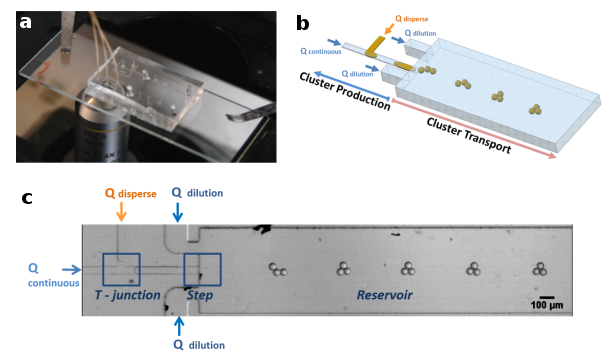
\includegraphics[width=0.9\columnwidth]{figs/microfluidic_channel.png}
 \caption{(a) Photo of a microfluidic channel placed above a desktop microscope. (b) Schematic of the channel geometry and generation of the droplet clusters. The main channel has a typical dimension of (50 $\mu$m $\times$ 600 $\mu$m $\times$ 5000 $\mu$m) in height, width, and length; hence, it can be considered as a Hele-Shaw cell. (c) Bottom view of the droplet self-assembly observed from the microscope. Pictures courtesy of Dr.\ Joshua Ricouvier. For more details, see   \cite{Shen_2016AS}.}
 \label{fig: chip}
\end{figure}


\section{Models and methods} \label{model}

\subsection{Hydrodynamic model}

The dynamics of two immiscible, Newtonian fluids in incompressible flows is governed by the Navier-Stokes equations
\begin{subequations}
 \begin{equation}
   \nabla \cdot {\bm u} = 0,
  \label{div free}
 \end{equation}
 \begin{equation}
      \frac{\partial {\bm u}}{\partial t} + {\bm u} \cdot \nabla {\bm u} = \frac{1}{\rho_iRe} \bigg(-\nabla p + \nabla \cdot \big[ \mu_i ( \nabla {\bm u} + \nabla {\bm u}^T ) \big] \bigg) + \frac{{\bm g}}{Fr},
  \label{NS}
 \end{equation}
\end{subequations}
where ${\bm u}$, $p$, $\bm{g}$, $\rho_i$ and $\mu_i$ denote the non-dimensional velocity, pressure, unit gravitational vector, density, and dynamic viscosity, respectively. Eq.\ \eqref{NS} is written for each fluid component, $i$ ($=1$ for the carrier fluid, 2 for the droplet), requiring a pressure boundary condition across the fluid interface
\begin{equation}
  p_2 - p_1 = \frac{\kappa}{Ca},
  \label{p laplace}
\end{equation}
with $\kappa$ being the mean curvature (the contribution due to the viscosity difference is neglected assuming matching viscosity \citep{Batchelor}).

So far, we have introduced three non-dimensional numbers: $Re$, $Ca$, and $Fr$, denoting the Reynolds, capillary, and Froude numbers, separately. Choosing fluid $1$ as the reference phase, they are defined as
\begin{equation}
  \begin{aligned}
    Re = \frac{\tilde{\rho}_1 \tilde{U} \tilde{L}}{\tilde{\mu}_1},\quad \quad Ca = \frac{\tilde{\mu}_1 \tilde{U}}{\tilde{\sigma}},\quad \quad Fr=\frac{\tilde{U}^2}{\tilde{g}\tilde{L}},      
  \label{non-di}    
  \end{aligned}
\end{equation}
where $\tilde{U}$, $\tilde{L}$, $\tilde{\rho}_1$, $\tilde{\mu}_1$, $\tilde{\sigma}$, and $\tilde{g}$ denote the reference \textit{dimensional} velocity, length, density, dynamic viscosity, surface tension, and gravitational acceleration. Following the experiments in   \cite{Shen_2016AS}, typical values of the reference velocity and length are $\tilde{U} \sim 100$ $\mu$m/s and $\tilde{L} \sim 100$ $\mu$m, leading to $Re \sim 10^{-2}$, $Ca \sim 10^{-5}$, and $Fr \sim 10^{-5}$ for oil-water systems. Therefore, inertial (but not gravitational) effects are negligible and the droplets shall remain mostly spherical. In the simulations that we are going to present, however, these numbers are enlarged within reasonable physical limits also to reduce the computation time. Specifically, $Re$ has been increased up to $10$ in most cases except those in Sec.\ \ref{sec:shear} (where $Re=1$) and those in Sec.\ \ref{sec:non-uniform} (where $Re=0.1$); $Ca$ is in the order of $10^{-3} \sim 10^{-2}$ depending on the $Re$; whereas $Fr=0.025$ if gravity is enabled (otherwise $\infty$). \xx{In general, the Reynolds number cannot be arbitrarily increased  as it is proportional to the fluid inertia. The reason we \textit{can} increase it here is essentially due to the uniformity of the underlying flow. In this case, the mere effect of further reducing the $Re$ is stretching the time scale, making the computations significantly longer. We have tested all cases at smaller $Re$'s to ensure that the differences are negligible in the case of fully developed Couette and Poiseuille flows.} This is discussed in more details in Appendix \ref{app:numerics}. 

Finally, we note that the surface tension can also vary due to temperature or surfactant concentration gradients, leading to Marangoni stress along the surface. The detailed chemistry is rather complex \cite{Eastoe}; in the present paper, we assume constant and uniform surface tension $\tilde{\sigma}$ to reduce the number of the governing parameters.

\subsection{Depletion theory}

\begin{figure}[t]
 \centering
 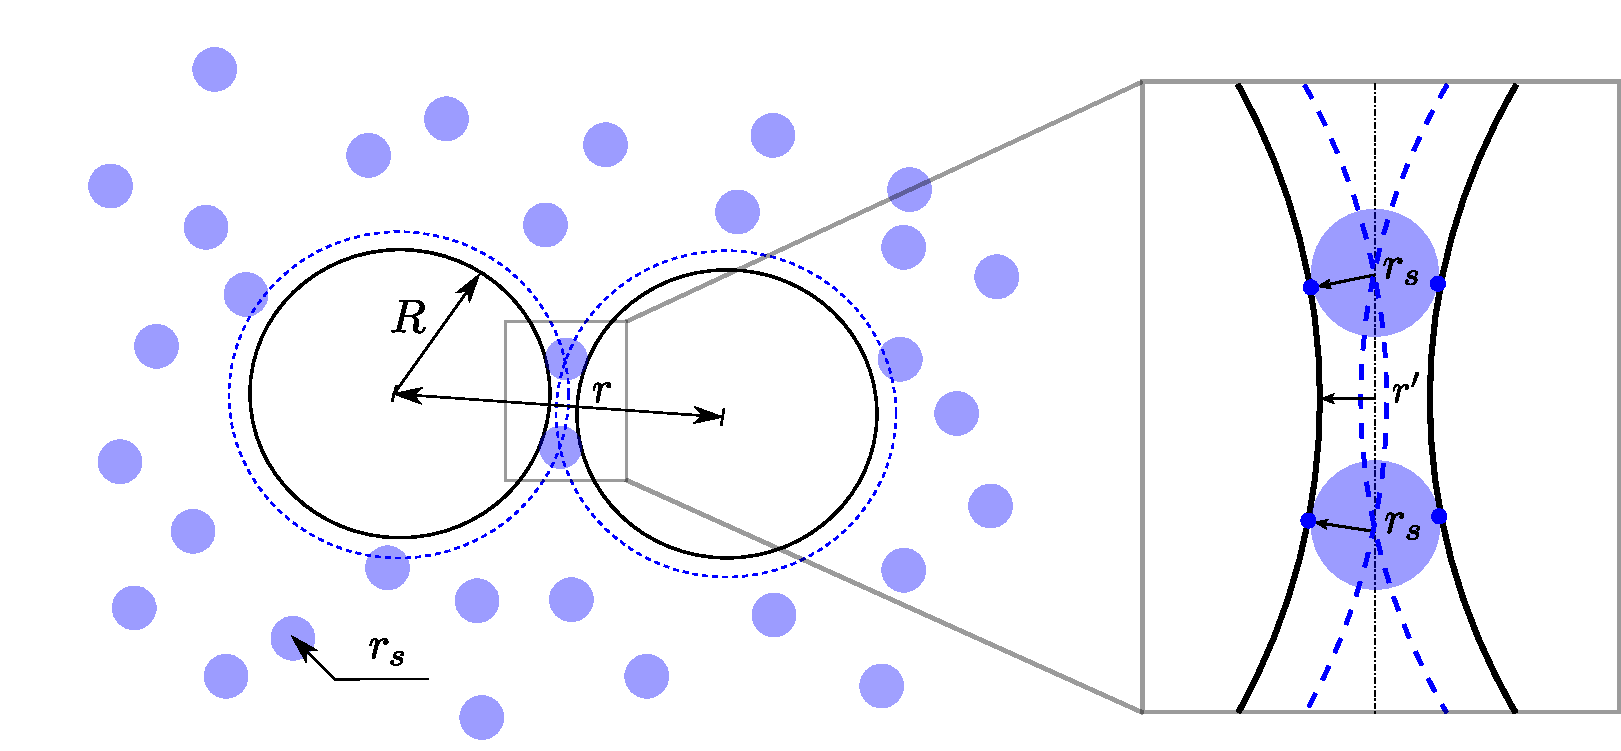
\includegraphics[width=0.9\columnwidth]{figs/depletion4.pdf}
 \caption{Depletion of surfactant micelles of radius $r_s$ between larger colloidal droplets of radius $R$, separated by distance $r$. The dashed lines around larger spheres represent the region from which the centers of small spheres are excluded. They overlap when $r \leqslant 2R+2r_s$. Inset: a zoom-in sketch of two droplets near contact.}
 \label{fig: depl theory}
\end{figure}

Droplets suspended in an ambient fluid dissolved by surfactant molecules typically experience an attractive depletion force. The first model to describe such interaction was proposed by  \cite{Asakura_Oosawa}, who assumed the surfactant micelles to be non-interacting hard spheres. As sketched in Fig.\ \ref{fig: depl theory}, a suspension of such small spheres around the large colloidal droplets creates an osmotic pressure on the droplet surface. When the distance between two droplets is less than the diameter of the surfactant micelles, the pressure defect due to the exclusion of the micelles pulls the drops even closer, corresponding to an attractive force. Integrating this force with respect to the inter-droplet distance $r$ leads to a potential energy
\begin{equation}
    U(r)=
    \begin{cases}
        \infty & \textrm{if} \quad r \leqslant 2R \\
        - p_{os}V_{ex} & \textrm{if} \quad 2R < r \leqslant 2R+2r_s  \\
        0 \quad & \textrm{otherwise}, \\
    \end{cases}
    \label{pot}
\end{equation}
where $V_{ex}$ is the excluded volume and $p_{os}$ is the osmotic pressure. For spherical droplets, $V_{ex}$ can be calculated analytically
\begin{equation}
    V_{ex}(r) = \frac{4\pi (R+r_s)^3}{3}\bigg[ 1- \frac{3r}{4(R+r_s)}+\frac{r^3}{16(R+r_s)^3} \bigg],
    \label{pot V}
\end{equation}
where $R$ and $r_s$ are, respectively, the radii of the big and small spheres. The osmotic pressure is given as
\begin{equation}
    p_{os} = nkT,
    \label{pot P}
\end{equation}
where $n$ is the number density of the small spheres, $k$ the Boltzmann constant, and $T$ the temperature. The negative sign in Eq.\ \eqref{pot} corresponds to the tendency of the system to reduce its potential energy as the overlap increases. This is equivalent to increasing the total entropy of the small spheres \citep{Melby_PRL_2007}, and it provides a physical description of the depletion force even when the droplets are deformable, or when $p_{os}$ cannot be expressed by the van't Hoff's formula (Eq.\ \eqref{pot P}) \citep{Asakura_Oosawa}.

Based on the above theory, we consider the depletion potential in the hydrodynamic model by adding an osmotic pressure, $p'(r')$, near the overlap region ($r'$ being the normalized distance to the droplet surface, see Fig.\ \ref{fig: depl theory}). Specifically, we write $p'$ as a Taylor-series expansion from $r'=r_s$
\begin{equation}
    p'(r'/r_s) = p'(1) + \bigg(\frac{r'}{r_s}-1 \bigg) \frac{\partial{p'}}{\partial{r'/r_s}},
    \label{pot P linear}
\end{equation}
with a constant $\partial{p'}/\partial{(r'/r_s)}$ satisfying the original depletion force acting on one droplet, i.e.
\begin{equation}
    -p_{os}A_{ex} = \int_\Omega \big(p'(1) - p'(r'/r_s)\big)dS,
    \label{pot P balance}
\end{equation}
where $A_{ex}$ is the effective area of the overlap $\Omega$. Note that, in this formulation, we do not require $p_{os}$ to be a thermodynamic pressure; instead, its strength can be defined by a non-dimensional number
\begin{equation}
    \Pi = \frac{p_{os}}{\kappa /Ca},
    \label{Pi}
\end{equation}
which normalizes $p_{os}$ by the Laplace pressure due to surface tension. Doing so, the osmotic pressure varies continuously within the overlap and depends linearly on $r'$. An expansion of the osmotic pressure with the distance corresponds to a gradient of the micelle concentration near the gap; and if the micelle is much smaller than the droplet, as it is in the microfluidic device of interest \citep{Shen_2016AS}, the gradient will be very sharp. Conversely, when the distance to the surface varies slowly, such as in the gap of a \xx{squeezed} droplet and a flat wall, a uniform pressure will be recovered. In essence, what we propose here is a method to model the osmotic pressure as an equivalent mechanical pressure such that a favorable pressure gradient from the center of the overlap region generates an outflow, pulling the droplets towards each other. This is clearly illustrated in Fig.\ \ref{fig: depl flow}, where two droplets approach each other due to the locally induced depletion flow.

\begin{figure}[t]
 \centering
 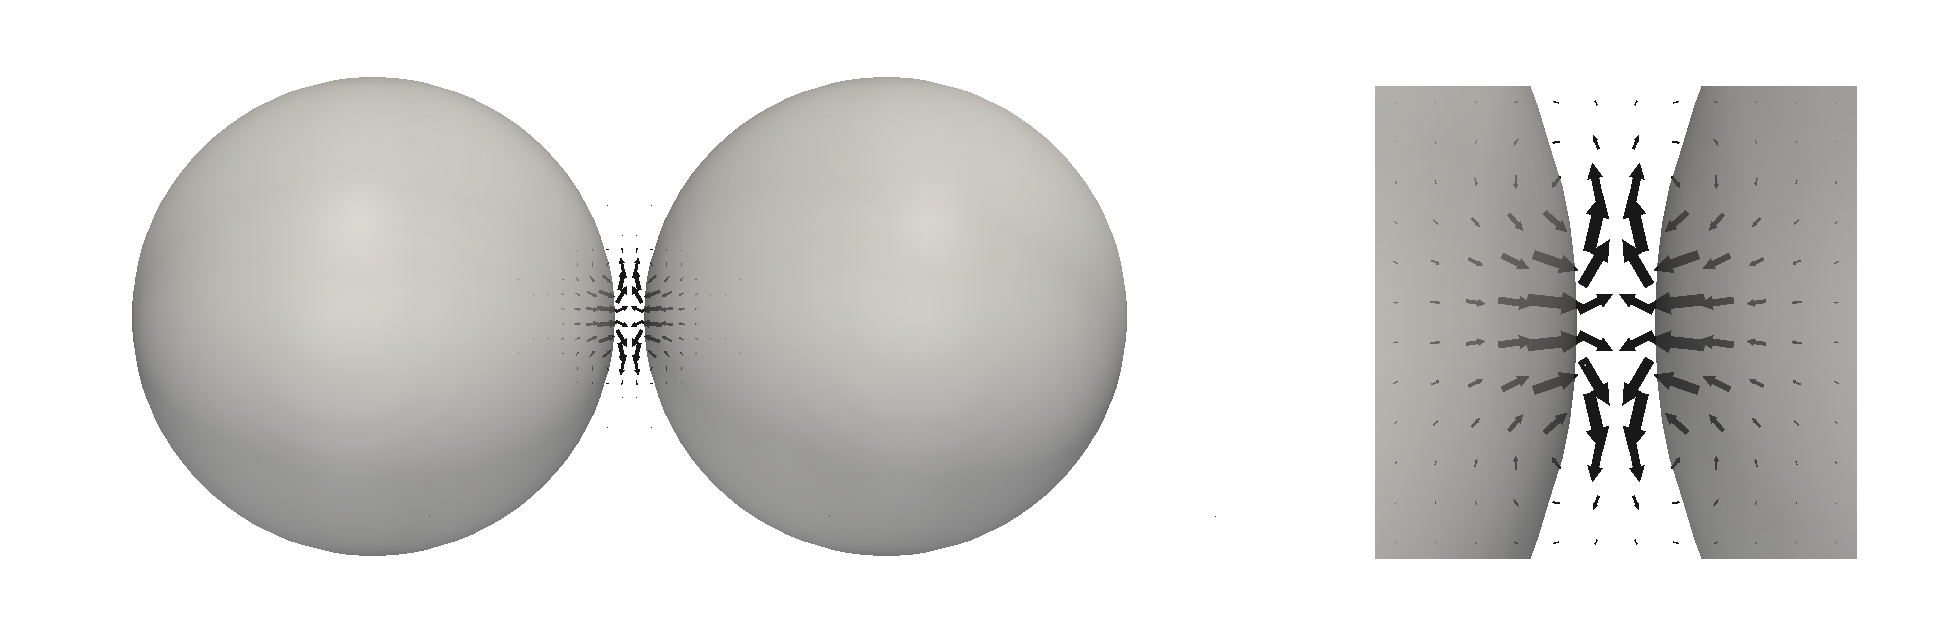
\includegraphics[width=0.9\columnwidth]{figs/depletion_flow.png}
 \caption{(left) Two droplets approaching in a quiescent flow, and (right) close-up of the flows in the gap due to the depletion force.}
 \label{fig: depl flow}
\end{figure}

\subsection{Numerical methods}

The above governing equations are solved numerically using the interface-correction level set/ghost fluid method (ICLS/GFM) \citep{ICLS}. The equations are discretized in space by the finite volume method, and integrated in time using the second-order Adam-Bashforth scheme. Combining several computational techniques, including the fast pressure correction method \citep{Dodd_JCP_2014}, the GFM \citep{Fedkiw_JCP_1999}, and the fast Fourier transform (FFT) \citep{Schumann_JCP_1988}, discontinuous quantities are treated sharply at high efficiency. For the detailed algorithm and validations, we refer to  \cite{ICLS}. The source code is also publicly available on GitHub \citep{icls_code}.

\section{Results}

In the following, we present simulation results of droplet motions in three types of flows: quiescent, shear-, and pressure-driven channel flows. In the last case, both Poiseuille flows and a non-uniform channel flow are considered. The purpose of using different flow types is to disentangle the effects of the depletion force, the droplet-droplet \xx{hydrodynamic} interaction, and the droplet-flow interaction. The simpler cases can be seen as model problems towards understanding of the more complex motions of droplet ensembles in realistic microfluidic devices.

\subsection{Approaching droplets in quiescent flows} \label{sec:quiescent}
\subsubsection{2 and 3 droplets}

\begin{figure}[t]
 \begin{center}
  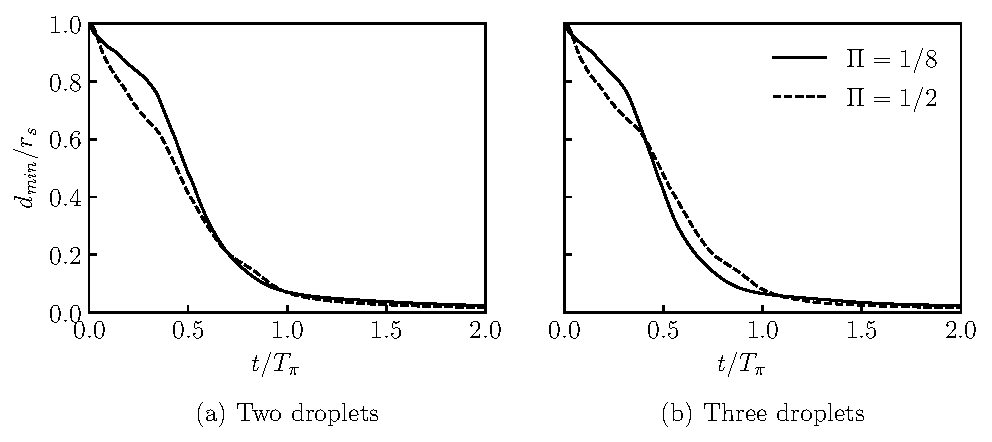
\includegraphics[width=\columnwidth]{figs/min_dist4.pdf}
  \begin{picture}(0,0)
   \put(-50,65){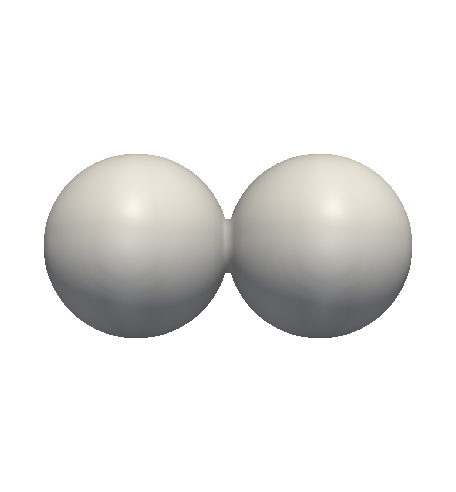
\includegraphics[height=1.5cm]{figs/2dp.png}}
   \put(120,65){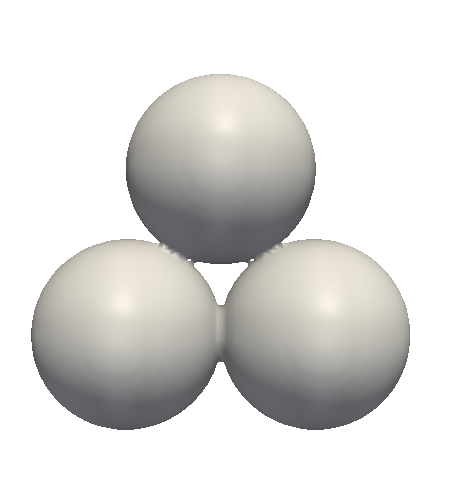
\includegraphics[height=1.5cm]{figs/3dp.png}}
  \end{picture}
 \end{center}
 \caption{Minimal distance between the droplet surfaces as function of time in the presence of depletion forces proportional to $\Pi=1/8$ (solid line) and $\Pi=1/2$ (dashed line). Simulation of (a) two droplets and (b) three droplets suspended in an initially quiescent fluid. Due to symmetry, only the minimal distance is plotted.}
 \label{fig: dep demo}
\end{figure}

The simplest case of droplet self-assembly is identical drops approaching in quiescent flows, i.e.\ no external flow motions. In such a case, the remaining fluid parameters can be grouped into two non-dimensional numbers, i) the Laplace number $La = \tilde{\sigma} \tilde{\rho}_1 (2\tilde{R})/\tilde{\mu}_1^2$, where $\tilde{R}$ is the droplet radius; and ii) the osmotic-to-Laplace pressure ratio $\Pi=p_{os}/p$. \footnote[3]{The density and viscosity ratios between the drop and the carrier fluids are assumed to be unity. See Appendix \ref{app:numerics} for the detailed numerical setup.} $La$ relates surface tension to the viscous stress, which can also be expressed as $La = Re/Ca$. $\Pi$ indicates the magnitude of the uniform osmotic pressure $p_{os}$ due to depletion of the surfactant micelles, scaled by a reference Laplace pressure $p$ due to surface tension (cf.\ Eq.\ \eqref{Pi}). In the following, we assume $La = 2000$ and $\Pi = 1/8$ or $1/2$, corresponding to the limit $Ca \ll Re \ll 1 $ and conditions above the critical micelle concentrations (CMC, see dimensional analysis below) as in the experiments \citep{Shen_2016AS}. 
%This is reasonable since Re $\sim 10^{-3}$ and Ca $\sim 10^{-6}$ (see \citep{shen_thesis}, pp 63-64), and the osmotic pressure at surfactant concentrations above CMC is of similar order-of-magnitude to the Laplace pressure (see dimensional values below). The same setup is used throughout the section, except that the domain size is adjusted to accommodate more droplets when necessary.

The approach of two and three droplets is illustrated in Fig.\ \ref{fig: dep demo}, where the minimal distance between the droplet surfaces $d_{min}$, normalized by the surfactant micelle radius $r_s$, is shown as a function of time. Here, time is re-scaled by the factor $T_\pi = \tilde{r}_s/(\tilde{R}\Pi)$ to account for the size contrast of the droplet and the surfactant micelle, thus indicating an inverse scaling of the approaching time with the osmotic pressure for inertialess droplets, i.e.\ $T \propto \Pi^{-1}$. Indeed, for both $\Pi = 1/8$ and $1/2$, our results show that $d_{min}$ approaches the limit of the grid spacing at $t \approx T_\pi$. The smooth approach in both cases and the collapse of the distance curves thus verify our modeling of the near field chemical interaction, consistent with an attracting depletion force. 
%Numerically, we let the droplets aggregate without applying any repulsion models, only to reduce the magnitude of $p_{os}$ when $d_{min}/r_s < 0.1$. 

We note that $T_\pi$ is not a physical time scale (it is dimensionless). One possible definition for the depletion time scale is $\tilde{\tau}_\pi = \tilde{r}_s \tilde{\mu}_1 /(\tilde{R} \tilde{p}_{os})$, which can be rewritten as $T_\pi Ca \tilde{\tau}$, with a convection time scale $\tilde{\tau} =2\tilde{R}/\tilde{U}$ in the range of $0.1$ to $1$ s typically. By substitution of usual values of colloidal systems, e.g. $\tilde{r}_s = 1$ nm, $\tilde{\mu}_1 = 10^{-3}$ kg/m-s, $\tilde{R} = 10$ $\mu$m, and $\tilde{p}_{os} = 100$ Pa (corresponding to surfactant micelles concentration of 5 CMC, see  \cite{shen_thesis}, p112), the estimated time scale is 1 ns. Although $\tilde{\tau}_\pi$ can be amplified by increasing the viscosity of the suspending fluid or reducing the micelles concentration, its magnitude is so small that the approaching can be considered instantaneous. Therefore, in practical microfluidic devices such as those in   \cite{Shen_2016AS}, one cannot expect to detect the dynamical approaching process due to depletion forces. The droplets will appear either bound or separated, depending on the surfactant concentration and flow conditions.

\subsubsection{4 to 10 droplets}

\begin{figure}[t]
 \centering
 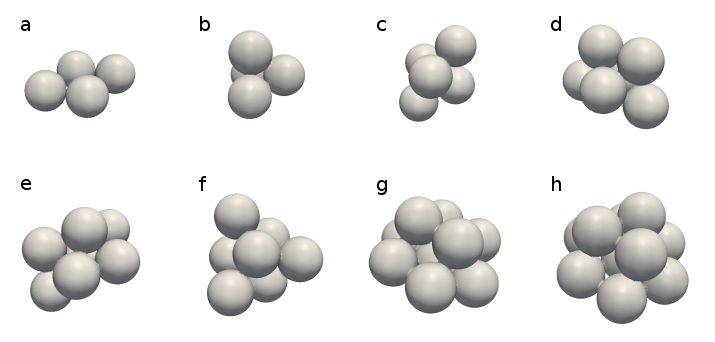
\includegraphics[width=0.9\columnwidth]{figs/packings.png}
 \caption{Packing of $N$ droplets due to the near field depletion force. (a-b) $N = 4$, (c) $N = 5$, (d) $N = 6$, (e) $N = 7$, (f) $N = 8$, (g) $N = 9$, (h) $N = 10$.}
 \label{fig: sph pack}
\end{figure}

To further demonstrate the effect of the depletion force, we ``virtually'' assemble four to ten droplets under various initial configurations to form stable clusters as illustrated in Fig.\ \ref{fig: sph pack}. These clusters can be either $2D$ or $3D$, exhibiting different levels/kinds of symmetry. In our simulations, the shape of the cluster is solely determined by the initial droplet arrangement, in the absence of any disturbance or other driving forces. Permitting disturbances, such as vibrations or thermal noises, would eventually lead to the formation of ``rigid clusters", i.e.\ clusters that cannot be reshaped by a small amount of inter-droplet displacement. Analytically, the number of possible rigid clusters grows rapidly with the number of droplets ($N$). For example, there is only one possible rigid cluster for $N = 4$, while there are 259 possibilities for $N = 10$, for packing of $3N-6$ contacts  \citep{Holmes-Cerfon}. For brevity, we only illustrate two examples for $N = 4$ (including one planar cluster) and one example for $N = 5$ to 10 in Fig. \ref{fig: sph pack}. 

We remind that the specific coordinates of the sphere packings bear no more significance than other possibilities in our simulations. They are arbitrarily chosen to illustrate the self-assembly due to the near field attraction. This is not the case for trapped equilibrium clusters, where less symmetric geometries are found to be favored by the entropic depletion force \citep{Meng2010,Klein2018}. \xx{Nor is it similar to colloidal particles interacting via short-range attracitve, long-range repulsive potentials, where complex phase transitions emerge depending on the competition of the interactions \citep{salr14,salr18}.} Here, the self-assembly is microfluidic-based, driven by the hydrodynamics rather than the minimization of free energy over long periods. We examine the effect of the flow next.

\subsection{Sticky droplets in shear-driven channel flows} \label{sec:shear}

When the droplets are carried by an external flow, their interactions are undoubtedly affected by the flow conditions, droplet-flow interactions and flow-induced droplet-droplet interactions \citep{Fouxon_2017}. To study these additional effects, we consider an elementary flow field, the wall-bounded simple shear flow, defined as $(u,v,w)=(0, \dot{\gamma}z,0)$ for $z \in [-L_z/2,L_z/2]$. Here, $v$ is the only non-zero velocity component, its magnitude varies linearly with the $z$ coordinate, and $\dot{\gamma}$ is the shear rate (see Fig.\  \ref{fig: shell}a). The presence of droplets will locally modify this flow field, which we sustain by enforcing opposite motions of two moving plates at $z= \pm L_z/2$.

Dating back to  \cite{Taylor501}, the deformation and motion of single or multiple droplet(s)/particle(s) have been studied extensively in simple shear flows \citep{lin_lee_sather_1970,batchelor_green_1972,batchelor_green_1972b,Zinchenko1983,Zinchenko1984,zurita-gotor_2007}. In the case of spherical particles/droplets, previously identified interaction modes include closed trajectories (particles rotate around each other in the vorticity plane), open-and-symmetric trajectories (particles return to their original $z$ positions after passing each other), and swapping trajectories (particles exchange the $z$ position after a binary encounter). The first two modes are generic features of a dilute suspension of particles or non-deforming/non-coalescing droplets, while the last mode arises when the particles are under relatively large geometric confinement. Conceivably, adding a near-field depletion force shall not alter these three modes as it is only activated at nearly touching, when the particles are already in a bound pair. What is yet to be explored, however, is when the gap between the two confining plates is smaller than the sum of the particle diameters (i.e.\ $L_z/D<2$), thus disabling the occurrence of the Batchelor-Green type of closed orbit.

\begin{figure}[t]
 \centering
 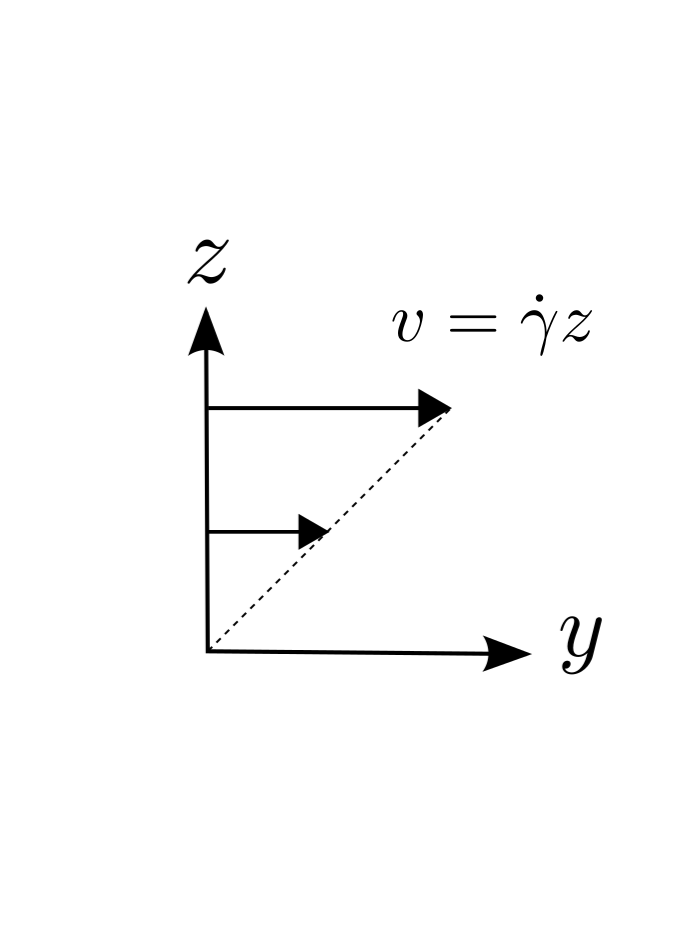
\includegraphics[width=.2\columnwidth]{figs/shear1.png}
 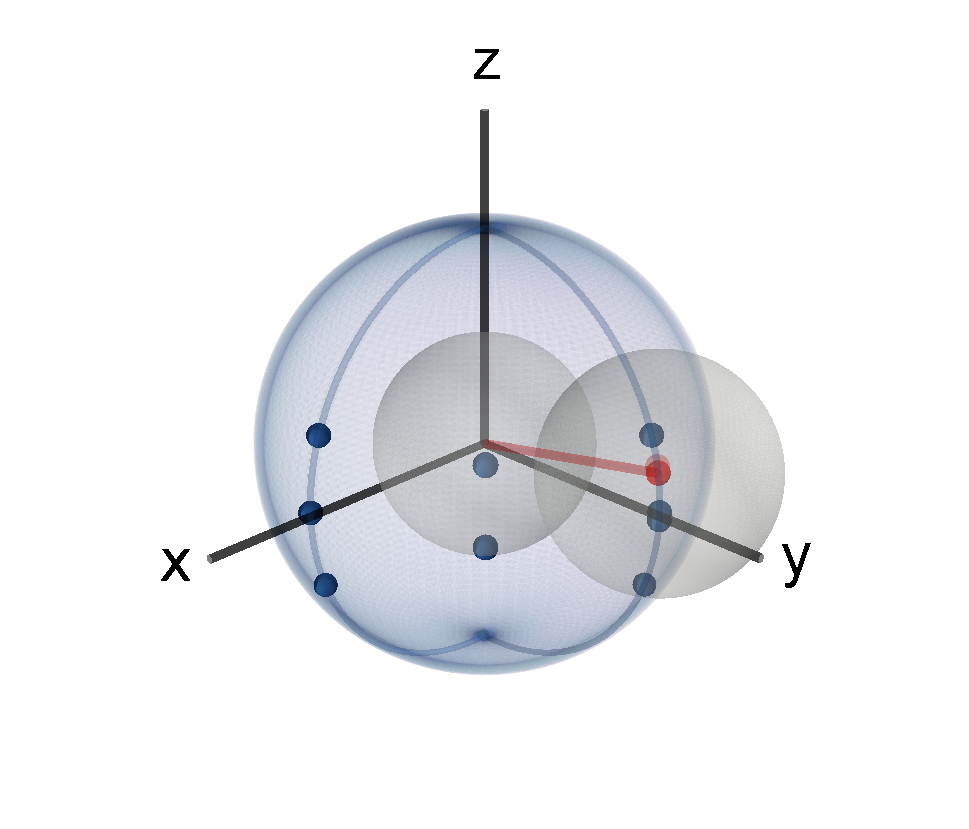
\includegraphics[width=.4\columnwidth]{figs/shell1.png}
 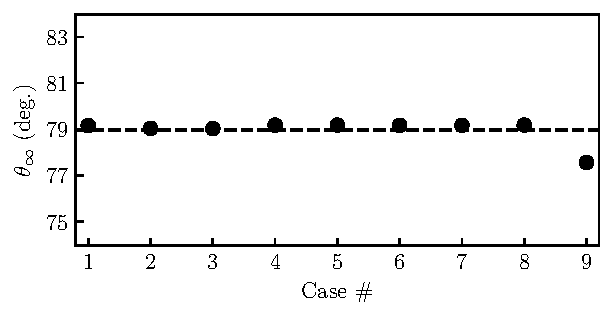
\includegraphics[width=.7\columnwidth]{figs/angle_final2.pdf}
 \begin{picture}(0,0)
   \put(-242,210){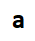
\includegraphics[height=.6cm]{figs/a.png}}
   \put(-242,110){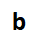
\includegraphics[height=.6cm]{figs/b.png}}
  \end{picture}
 \caption{Stable configuration of a droplet pair in the simple shear flow. (a) Spherical diagram of the initial (blue dots) and final (red dots) positions of the second droplet in the reference frame of the first droplet. The blue arcs mark the border of the first quadrant where nine initial positions are considered. The undisturbed flow is a simple shear in the $yz$ plane. (b) Steady-state polar angle, $\theta_\infty$, corresponding to the cases in Table \ref{tbl: cases}. The average value is 79 deg. (dashed line). The stable azimuthal angle is identically 0.}
 \label{fig: shell}
\end{figure}

\begin{table}[h]
  %\small
  \centering
  \caption{\ Initial polar ($\theta$) and azimuthal ($\phi$) angles of the second droplet in the reference frame of the first droplet. $\theta$ and $\phi$ are measured from the $z$- and $x$-axes, respectively (see Fig.\ \ref{fig: shell}(a)).}
  \label{tbl: cases}
  %\begin{tabular*}{0.48\textwidth}{@{\extracolsep{\fill}}l rrrrrrrrr}
    \tabulinesep=1.2mm
    \begin{tabular}{ l rrrrrrrrr}
    \hline
    Case \# & 1&2&3&4&5&6&7&8&9 \\
    \hline
    $\theta$ (deg.) & 70&70&70& 89&89&89& 91& 110&110 \\
    $\phi$   (deg.) & 90&45& 0& 90&45& 0& 90&  90&  0 \\
    \hline
  \end{tabular}
\end{table}

Fig.\ \ref{fig: shell}(a) illustrates various initial conditions of two touching droplets, corresponding to the nine cases listed in Table \ref{tbl: cases}, at $L_z/D=1.5$. Specifically, the initial positions of the second droplet is given in the spherical coordinates centered at the first one, where all cases are located in one quadrant-sphere as we do not distinguish between the two droplets (the rest are equivalent due to symmetry). Contrary to the less confined conditions where a bound pair would rotate indefinitely relative to each other under shear \citep{batchelor_green_1972,Zinchenko1984}, Fig.\ \ref{fig: shell} shows that the droplets tend to reside in the vorticity plane (i.e.\ the $yz$ plane) with a stable polar angle $\theta_\infty \approx 79$ deg. This is true even if the two droplets are not initially in the same vorticity plane (case 2,3,5,6,9), or if the second droplet is in the lower hemisphere relative to the first one (case 7,8,9). Particularly, in cases 8 and 9, the droplet pair first rotates clockwise, then slides along the wall, before finally reaching the stable orientation (see ESI Video 1). The anomalous trajectory is a clear evidence of the influence of the walls, which, together with the attractive depletion force, break the symmetry of the droplet binary interactions.

The above results suggest that, for two droplets subject to an attractive depletion force in strongly confined simple shear flows, only one configuration is dynamically stable. It further implies that, for multiple droplets ($N>2$) traveling in a pressure-driven channel with $H/D<4$ ($H$ being the channel height, see Sec.\ \ref{sec:channel}), a chain-like structure oriented in the flow direction is expected. We remark that the precise configuration of the droplet cluster may depend on the flow conditions and the level of confinement (see Appendix \ref{app:trajectory} for further discussion); however, the \textit{qualitative} picture of the pairwise interaction shall remain unchanged, provided that the number of contact is $N-1$. As this is often the case before a compact cluster is formed, we proceed to examine the droplet self-assembly in pressure-driven flows.


\subsection{Droplet clusters in pressure-driven channel flows} \label{sec:channel}

\xx{In the following, clusters of three or four droplets are initialized to be in contact ($N-1$ contacts for $N$ droplets) and are released into different regions of a microfluidic channel to study their transport behavior. The production of these droplets is omitted, as the step-emulsifier is typically much smaller than the size of the channel, allowing for separation of the two processes \citep{shen_thesis,step-emuls}. We note that, although the droplets are already in a cluster initially, their relative rearrangement is still important as it determines the cluster morphology in the final state. The latter results primarily from the droplet-flow interaction and has direct consequence on the photonic properties of the droplet lattice, as we will discuss in details below.}

\subsubsection{Uniform region (the Poiseuille flow)} \label{sec:poi}

\begin{figure}[t]
 \centering
 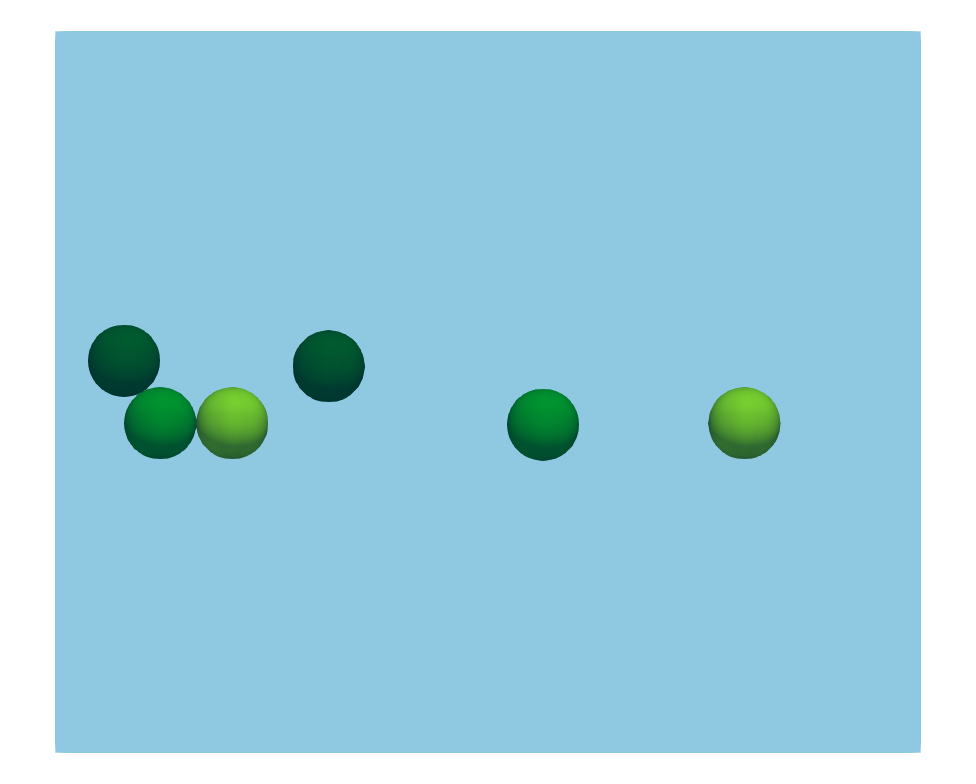
\includegraphics[width=.3\columnwidth]{figs/3-scatter-top.png}
 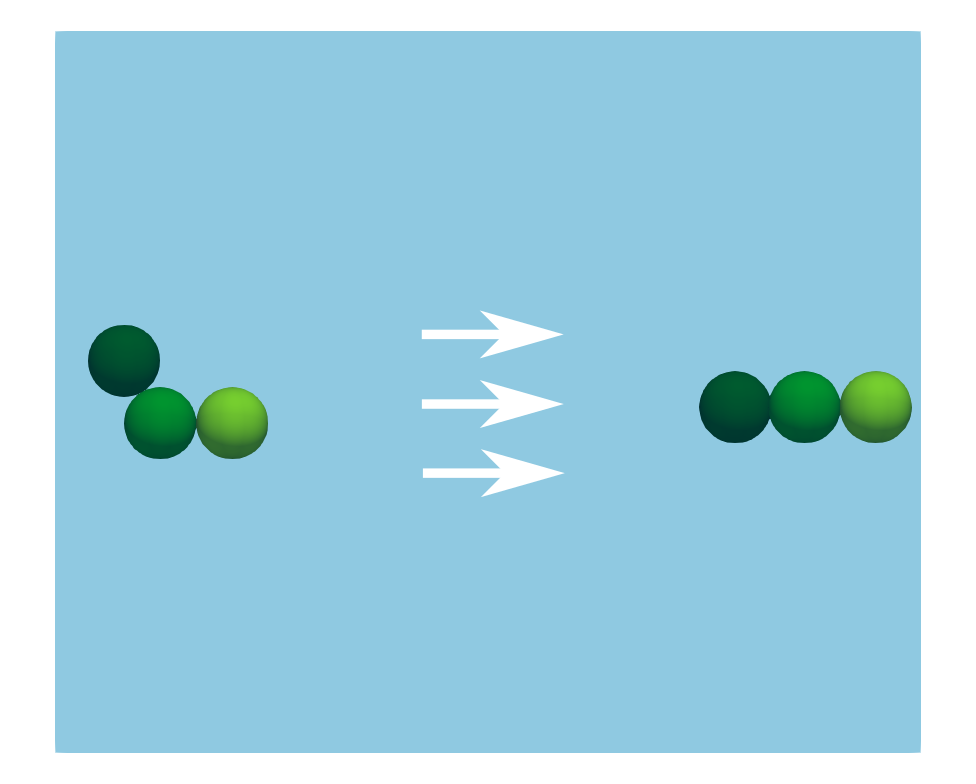
\includegraphics[width=.3\columnwidth]{figs/3-line-top1.png}
 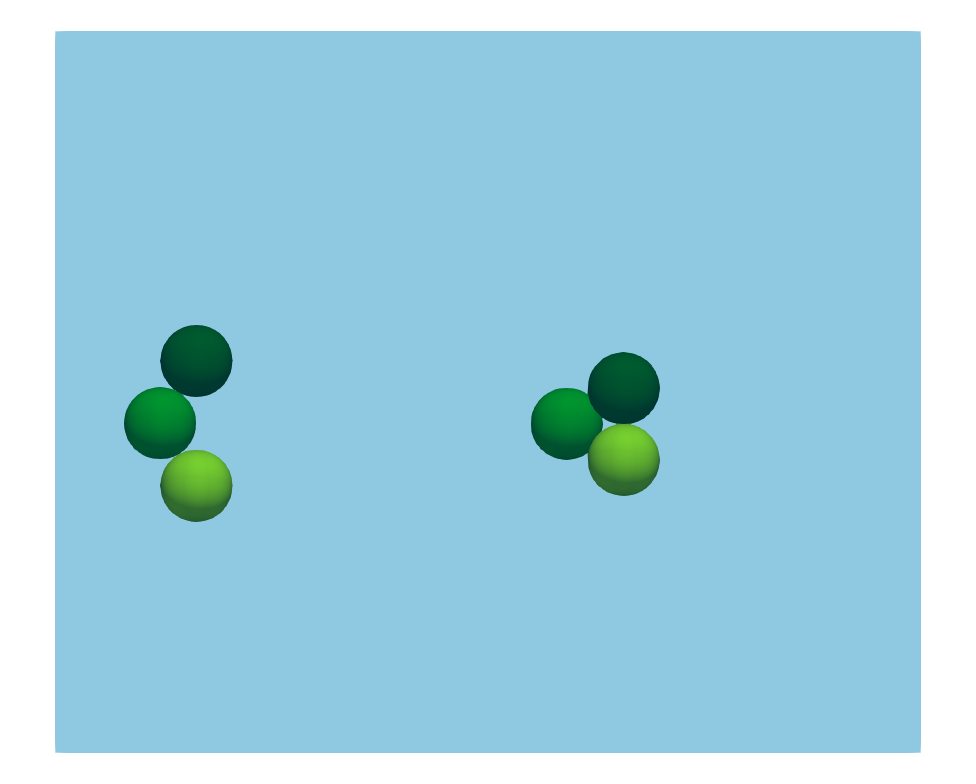
\includegraphics[width=.3\columnwidth]{figs/3-triangle-top.png}
 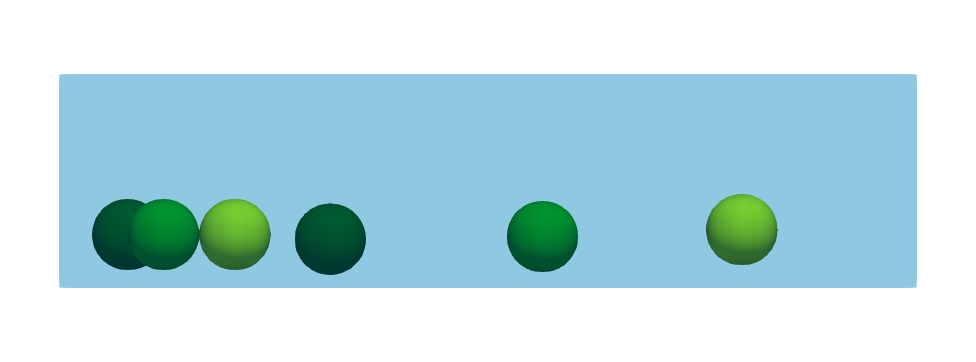
\includegraphics[width=.3\columnwidth]{figs/3-scatter-side.png}
 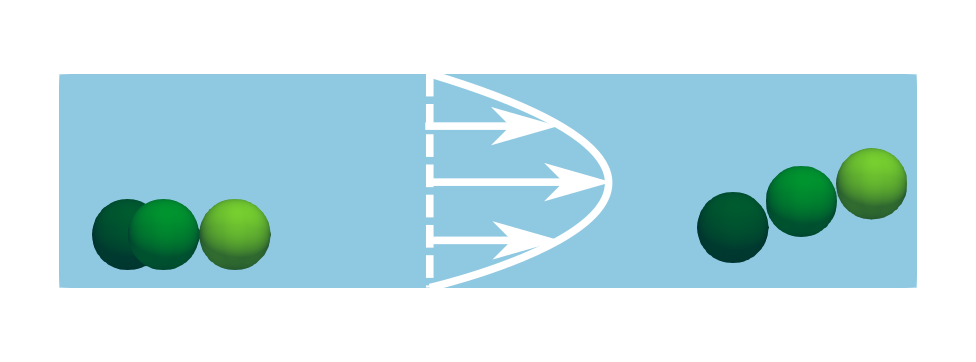
\includegraphics[width=.3\columnwidth]{figs/3-line-side1.png}
 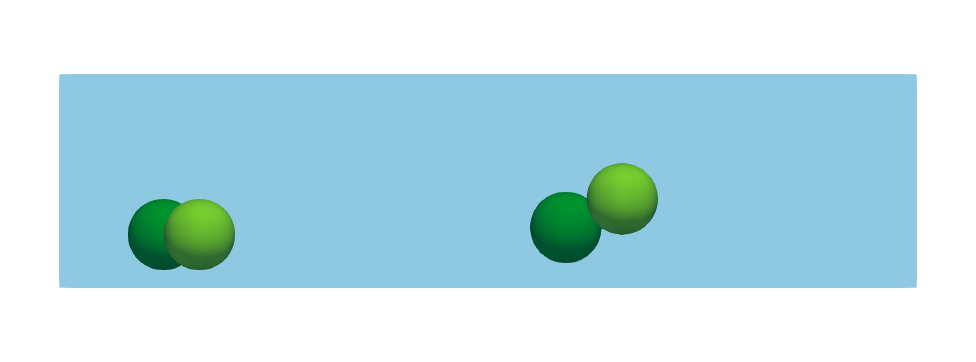
\includegraphics[width=.3\columnwidth]{figs/3-triangle-side.png}
 %\includegraphics[width=.9\columnwidth]{figs/result_poi.pdf}
 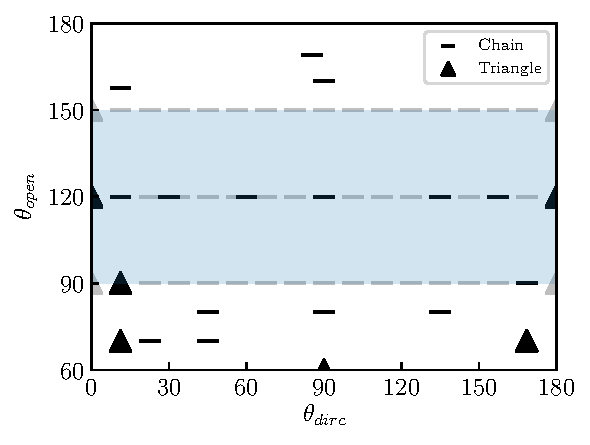
\includegraphics[width=.6\columnwidth]{figs/result_poi1.pdf}
 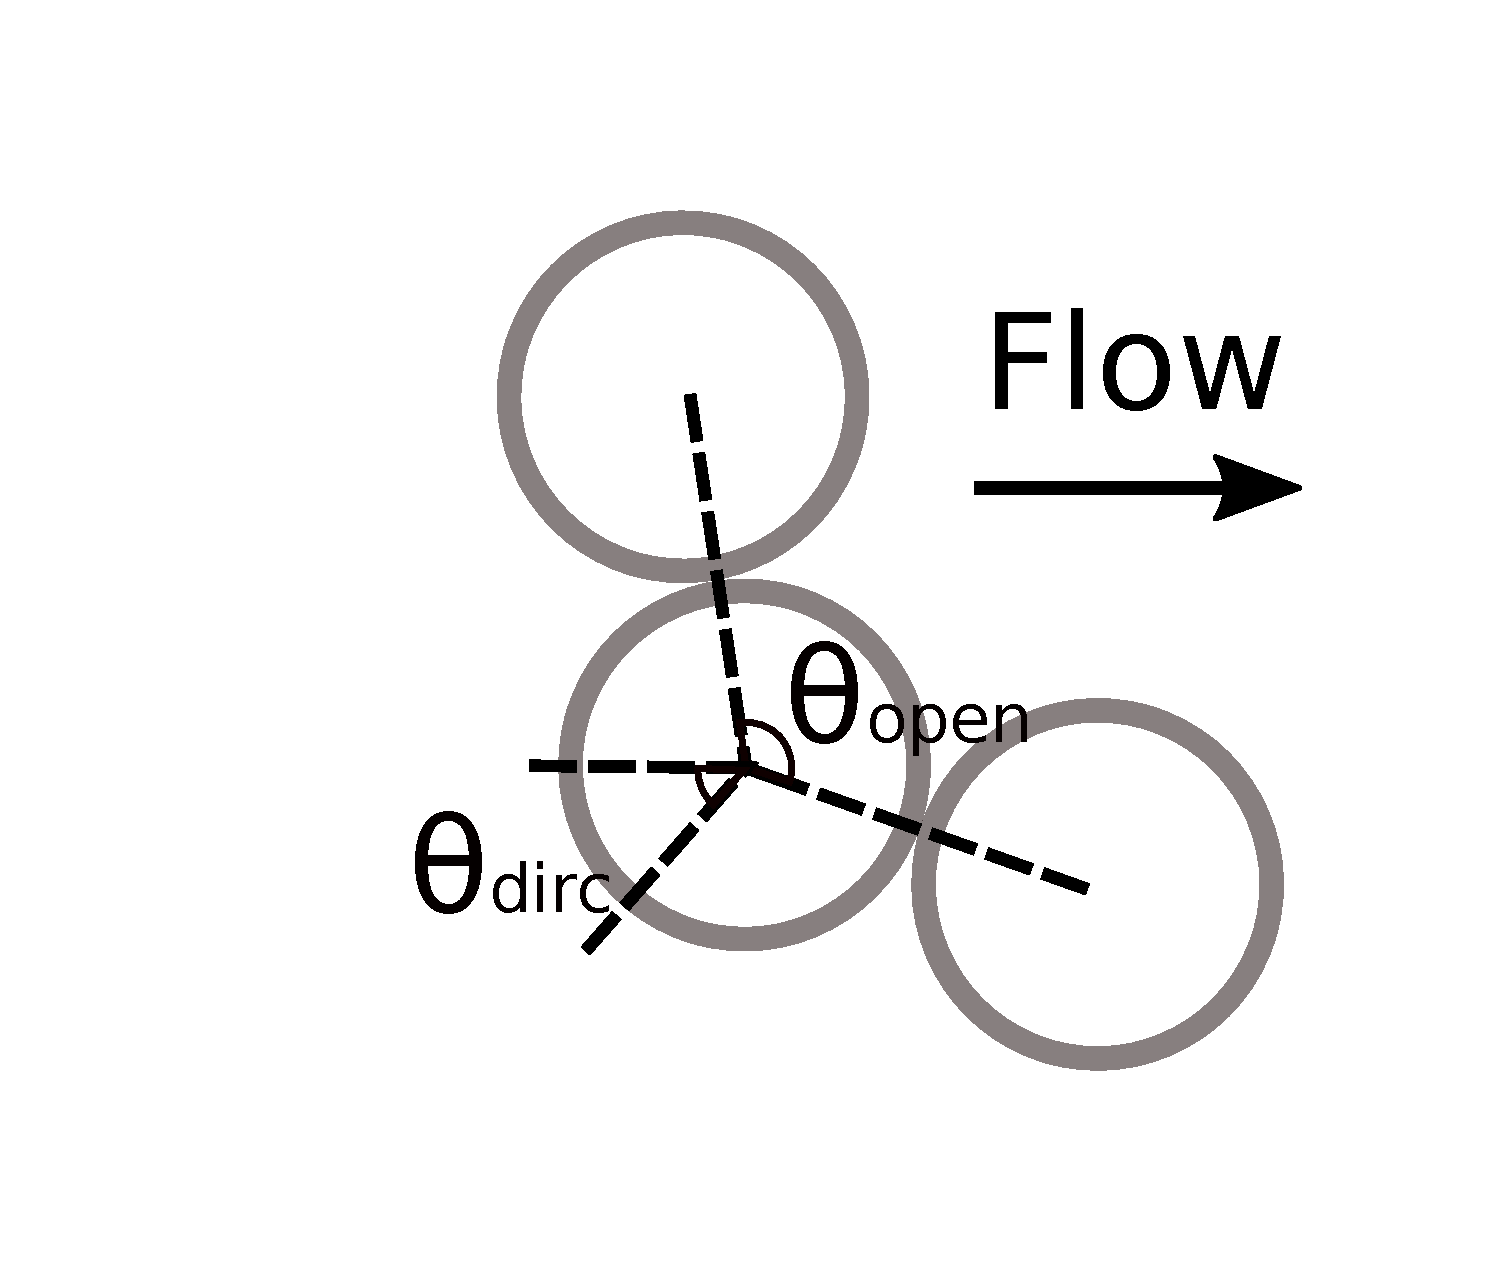
\includegraphics[width=.3\columnwidth]{figs/angle_sketch1.pdf}
 \begin{picture}(0,0)
   %\put(-180,75){\includegraphics[height=1.4cm]{figs/angle_sketch.pdf}}
   \put(-100,75){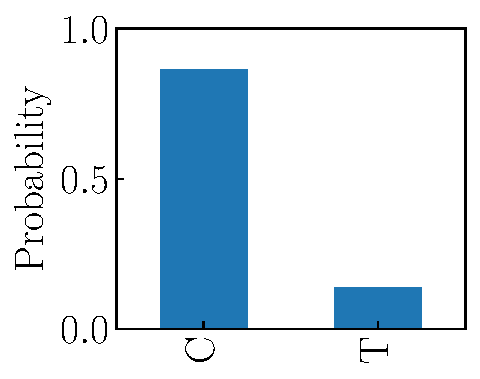
\includegraphics[height=2.5cm]{figs/result_poi_bar.pdf}}
   \put(-325,260){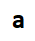
\includegraphics[height=.6cm]{figs/a.png}}
   \put(-325,140){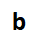
\includegraphics[height=.6cm]{figs/b.png}}
 \end{picture}
 \caption{Three droplets in the Poiseuille flow. (a) Top (upper panels) and side (lower panels) views of the droplet positions. The droplets are colored differently only for visualization purposes. Left: without any depletion force (scattered droplets). Middle: with depletion force (forming a chain). Right: with depletion force (forming a triangle due to a different initial configuration). (b) Phase diagram showing the final configuration of three droplets under depletion force. $\theta_{open}$ and $\theta_{dirc}$ denote the \xx{initial} opening and the direction angles (see inset for illustration). \xx{Interpolating the results for $\theta_{open} \in [90,150]$ (shaded region), chain is clearly the predominant structure as shown in the probability distribution.}}
 \label{fig: poi results}
\end{figure}

First, we consider droplet clusters in a Poiseuille flow; that is, we place the droplets in a channel whose undisturbed velocity is given as $(u,v,w)=(0,6z/H(1-z/H),0)$, with the channel height $H=3D$. As in the simple shear flow, the droplets are neutrally buoyant, and $x$, $y$, $z$ denote the spanwise, streamwise, and wall-normal directions, respectively. Enforcing periodic boundary conditions in both $x$ and $y$ directions, the flow can be computed efficiently using FFT, approximating the flow field far from the edges of the Hele-Shaw channel (see Fig.\ \ref{fig: chip}b).

As a control case, we simulate three droplets initially located near the bottom of the channel without any depletion forces. This is shown in the first column of Fig.\ \ref{fig: poi results}a, where the top and bottom panels illustrate the top and side views of the channel (see Fig.\ \ref{fig: chip}). The two snapshots are separated by $13.5$ convection time units (i.e.\ $\tilde{\tau}$). Clearly, the droplets quickly scatter as carried by the flow. In a previous work, we theoretically predicted the emergence of singlets and pairs of a dilute particle suspension due to weak particle-particle interactions \citep{Fouxon_2017}. This example illustrates the separation of a droplet cluster, enhanced by their initial proximity already at $N=3$, supporting our theoretical predictions.

In contrast, when the droplets are bound by a strong depletion force, the same initial condition can lead to a chain structure oriented in the flow direction, see the second column of Fig.\ \ref{fig: poi results}a. Inspection of the side view reveals the apparent reason: the leading droplets migrate towards the middle of the channel due to the shear, thus experiencing faster flows; the attractive depletion force prevents the cluster from separating into singlets and pairs, yielding the eventual droplet string parallel to the stream. We propose that this shear-induced alignment mechanism is fundamentally due to the confinement-mediated pairwise interaction discussed in the previous section. The difference is that the Poiseuille flow has no simple analytical solution in the presence of droplets (hence the two cannot be compared exactly), and the confinement requirement is halved due to the symmetry of the parabolic velocity profile.

To further test the robustness of the shear-alignment mechanism, we consider multiple initial configurations of the triplet in the same flow. As sketched in Fig.\ \ref{fig: poi results}b, three touching droplets whose centers are in the same $xy$ plane can be completely described by two angles: $\theta_{open}$, denoting the opening angle of the triplet, and $\theta_{dirc}$, denoting the angle between the bisector of the triplet and the direction of the undisturbed flow. For identical droplets, admissible angles are $\theta_{open} \in [60, 180]$ deg., and $\theta_{dirc} \in [0,180]$ deg. Extensive tests show that the chain structure is far more favorable than the closed triangular cluster in Poiseuille flows \xx{(see Fig.\ \ref{fig: poi results}b)}. One case of the triangle cluster is visualized in the third column of Fig.\ \ref{fig: poi results}a, where two droplets initially on the sides migrate towards the center, eventually leading to the closure of the open chain. In the vast majority of the cases, however, a straight droplet string aligned with the flow is observed, even if they are close to a triangle initially (note the small $\theta_{open}$ cases in Fig.\ \ref{fig: poi results}b).

The above results confirm that the chain-like structure is indeed the predominant configuration of droplets bound by short-range depletion forces in the Poiseuille flow. Experimentally, this corresponds to strong diluting flows at the channel inlet, where long droplet strings are also observed further downstream (see  \cite{shen_thesis}, p137). More importantly, our simulations suggest that aligning of the droplets is a $3D$ shear-induced effect mediated by the confinement. The cross-stream migration of the droplets happens within a much shorter time span than any tangential rearrangement due to the dipolar interactions (cf.\  \cite{Diamant} and  \cite{Fouxon_2017}). This is one key difference between our $3D$ microfluidic channel and other $q2D$ devices. 


\subsubsection{Entry region (with a non-uniform inflow)} \label{sec:non-uniform}

\begin{figure}[t]
 \centering
 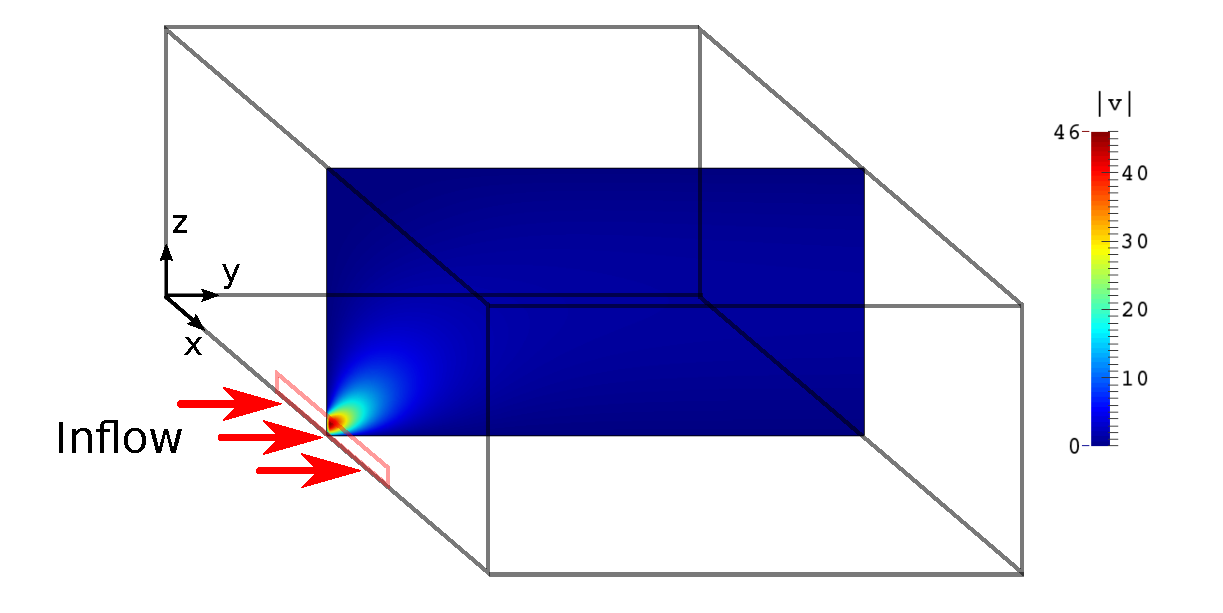
\includegraphics[width=.9\columnwidth]{figs/non-uniform_inflow1.pdf}
 \caption{\xx{Cross-section of the channel inlet and magnitude of the initial velocity field at the central plane without droplets. The flow is injected from the step-emulsifier (red rectangle), where the droplets (not shown) are produced, into the channel (cf.\ Fig.\ \ref{fig: chip}b). The velocity is normalized such that $\abs{v}=1$ corresponds to the bulk flow velocity averaged over the entire channel.}}
 \label{fig: non-uniform sketch}
\end{figure}

So far, we have showed i) the self-assembly of two to ten droplets in quiescent flows, ii) the alignment of a droplet pair in confined simple shear flows, and iii) the chaining (or, sometimes clustering) of a triplet in the Poiseuille flow. Of these, i) is caused solely by the near-field depletion force, and provides the necessary condition for ii) and iii); ii) and iii) are closely related, and in principle can be generalized to clusters of $N>3$. In addition, we have distinguished our $3D$ channel from typical $q2D$ ones. The remaining question is what makes the droplets self-assemble into compact clusters within short distances (i.e.\ $\sim \mathcal{O}(10D)$ \footnote[4]{Dipolar interactions under similar confinement require at least $\mathcal{O}(100D)$ distance to see any clustering effect, see \cite{Fouxon_2017}.}) as seen in the experiment of   \cite{Shen_2016AS}?

To answer this question, we perform series of simulations of a triplet/quadruplet cluster in a non-uniform channel, similar to the actual entry region of the microfluidic channel (see Fig.\ \ref{fig: chip}). Fig.\ \ref{fig: non-uniform sketch} illustrates the cross-sectional design of the channel inlet and the obtained velocity distribution in the central plane. Specifically, the computational domain has a size of $(L_x/D,L_y/D,L_z/D)=(4.5,6,3)$ or $(4.5,8,3)$ depending on the cases, and the ratio of the inflow area to the entire cross-section is $A_{in}/A_{tot}=1/32$, resulting in a highly non-uniform velocity profile. Near the inlet, the peak velocity reaches 46 times the average bulk velocity, then quickly smoothens downstream. To utilise the efficient FFT solver, we again use periodic boundary condition in the spanwise ($x$) direction, mimicking the effect of diluting flows on the sides. The droplet-to-carrier-fluid density ratio is $\tilde{\rho}_2/\tilde{\rho}_1=1.8$, corresponding to silicone oil in water. The rest of the governing parameters are $Re=0.1$, $Ca=0.025$, $Fr=0.0027$, and $\Pi=1$.

\begin{figure}[t]
 \centering
 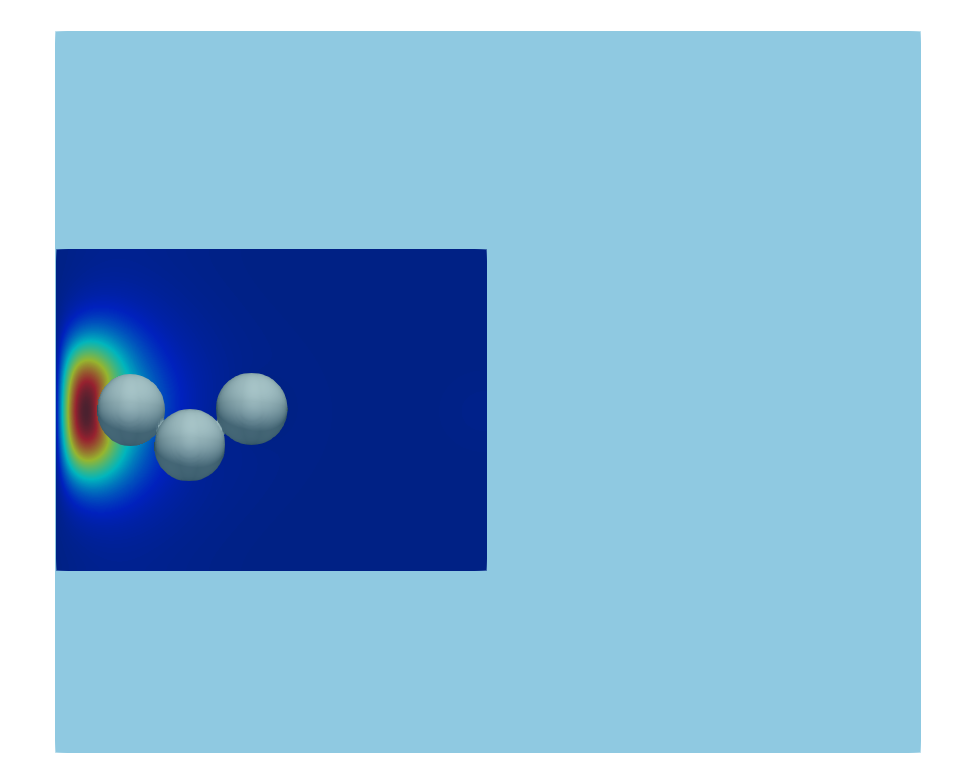
\includegraphics[width=.3\columnwidth]{figs/bx4-top-2k_s.png}
 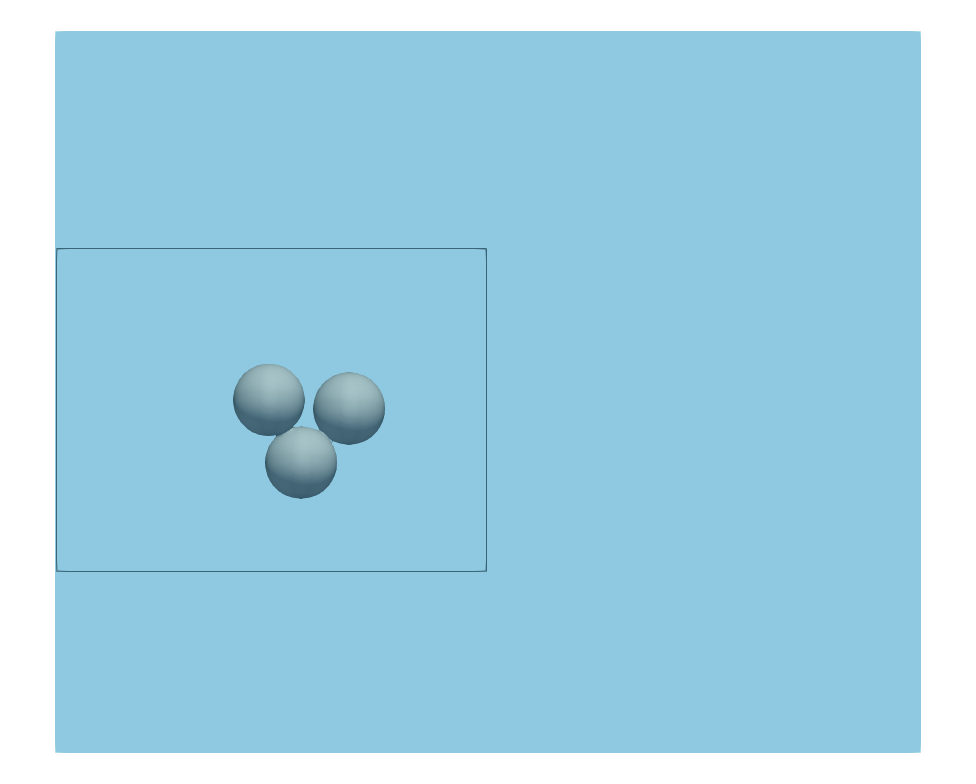
\includegraphics[width=.3\columnwidth]{figs/bx4-top-140k.png}
 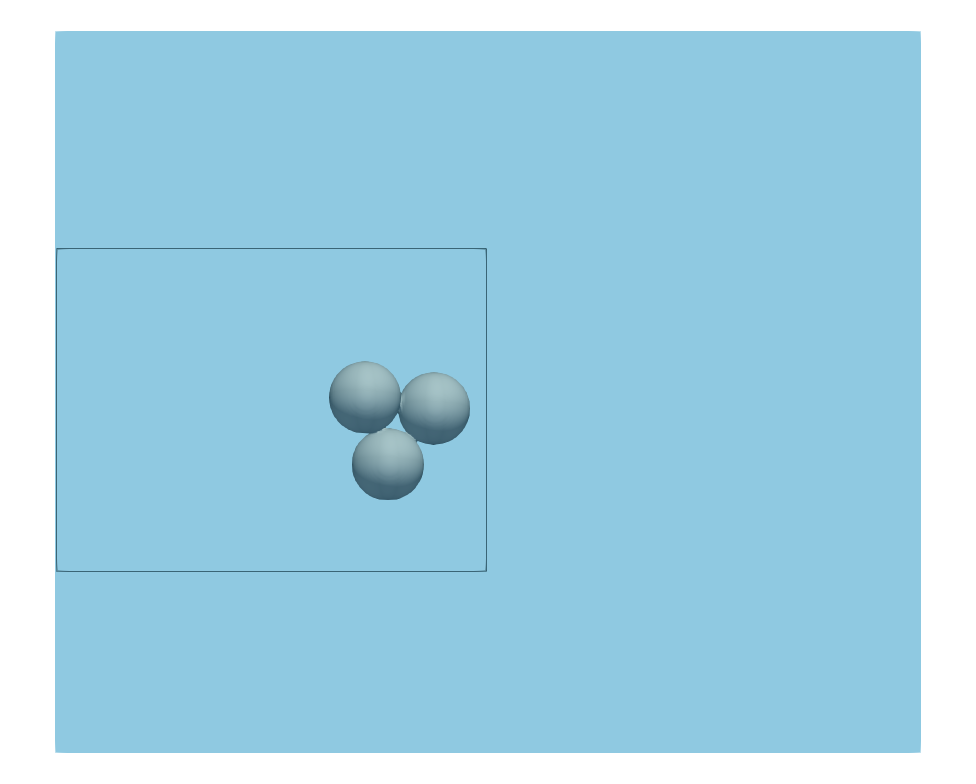
\includegraphics[width=.3\columnwidth]{figs/bx4-top-280k.png}
 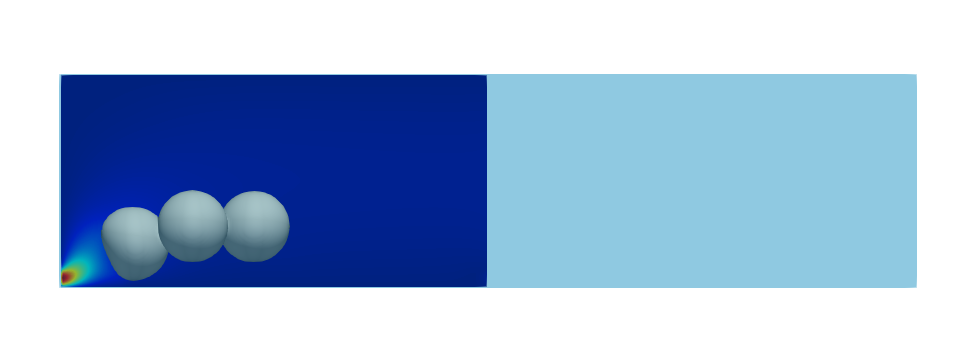
\includegraphics[width=.3\columnwidth]{figs/bx4-side-2k_s.png}
 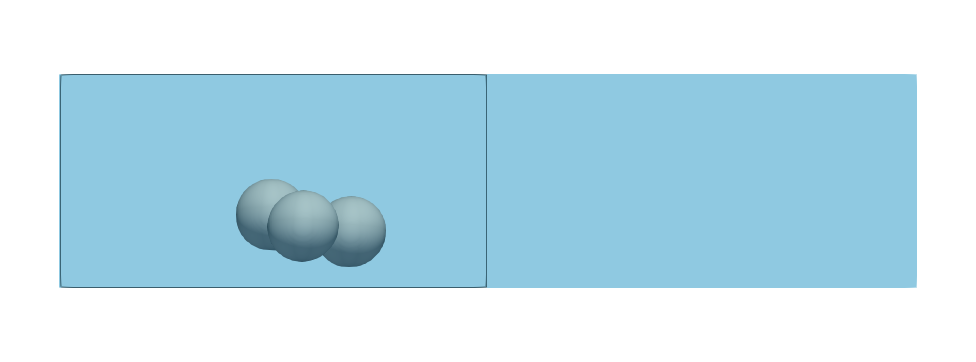
\includegraphics[width=.3\columnwidth]{figs/bx4-side-140k.png}
 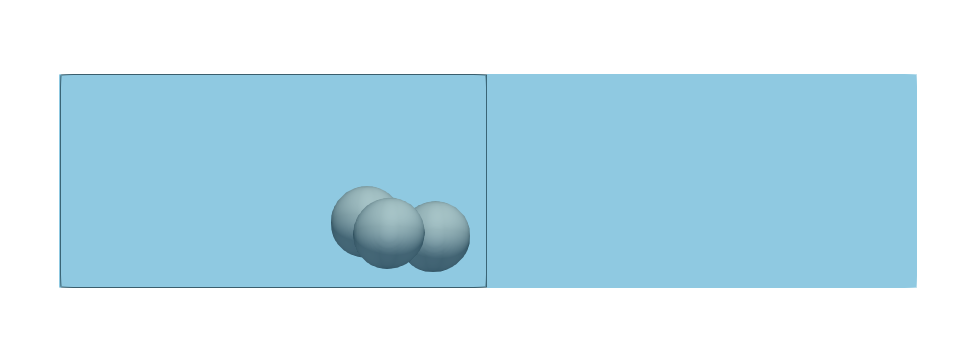
\includegraphics[width=.3\columnwidth]{figs/bx4-side-280k.png}
 
\includegraphics[width=.75\columnwidth]{figs/time_arrow.pdf}
 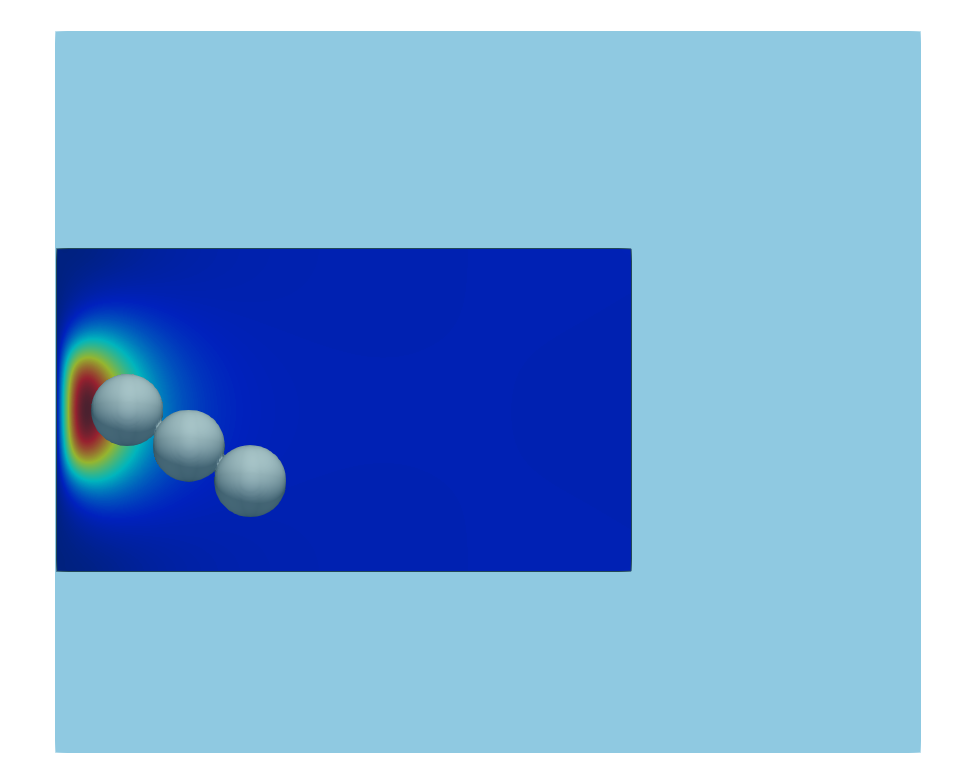
\includegraphics[width=.3\columnwidth]{figs/bx6-top-0.png}
 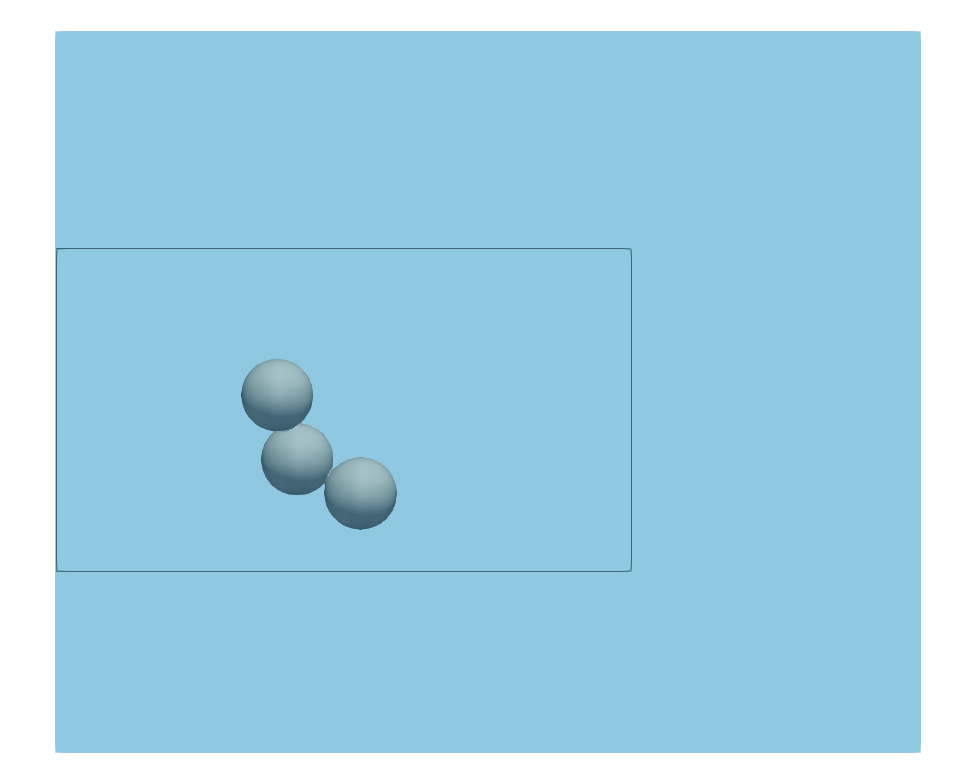
\includegraphics[width=.3\columnwidth]{figs/bx6-top-150k-l.png}
 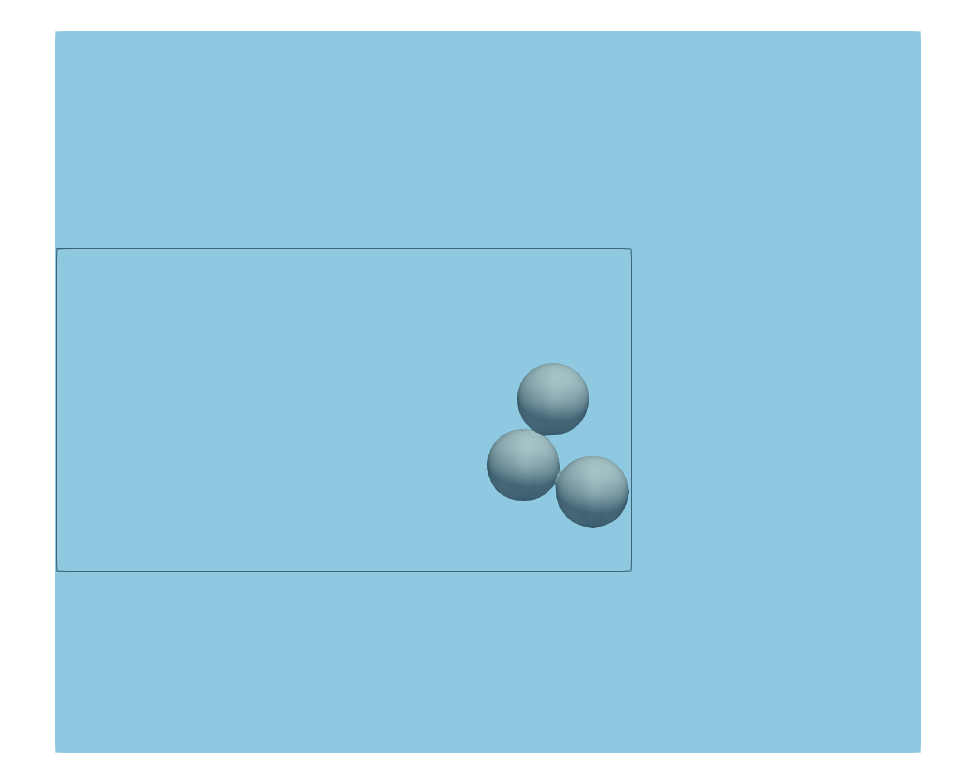
\includegraphics[width=.3\columnwidth]{figs/bx6-top-570k.png}
 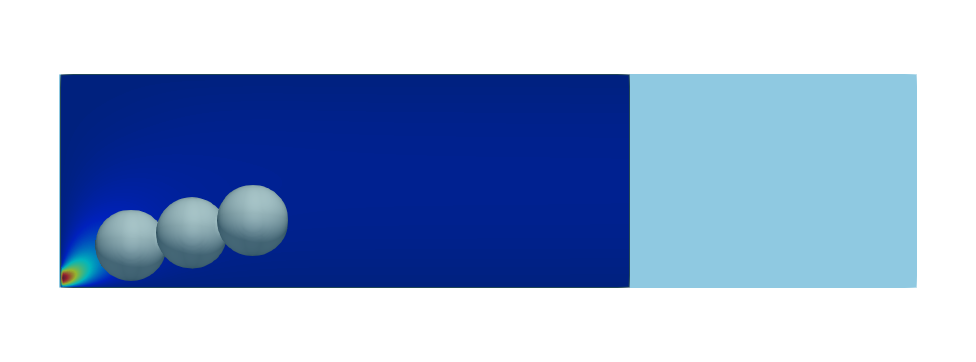
\includegraphics[width=.3\columnwidth]{figs/bx6-side-0.png}
 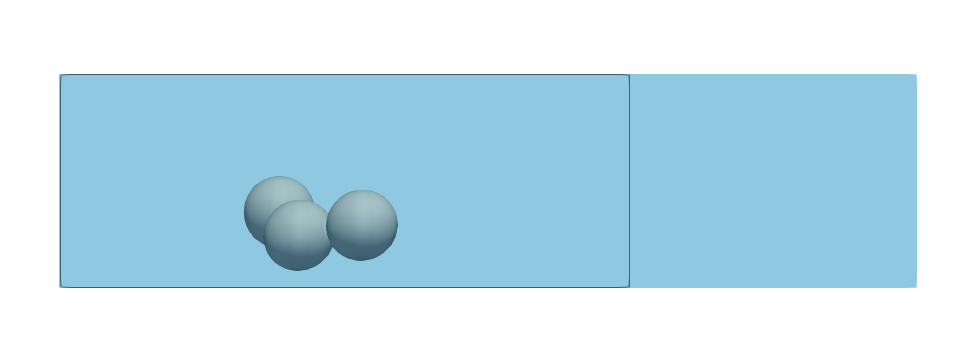
\includegraphics[width=.3\columnwidth]{figs/bx6-side-150k-l.png}
 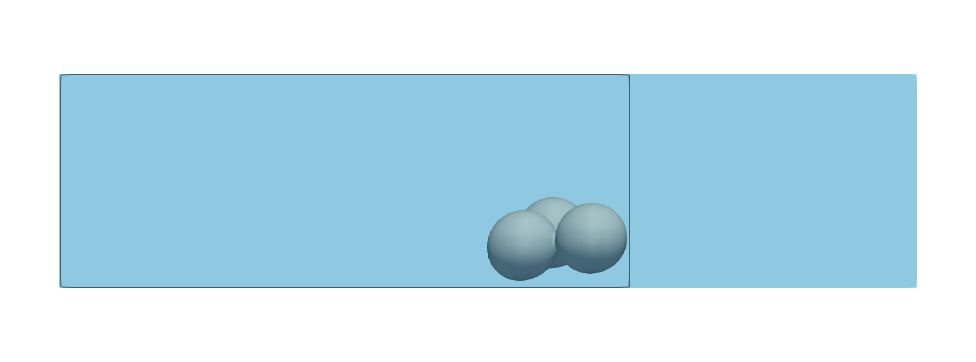
\includegraphics[width=.3\columnwidth]{figs/bx6-side-570k.png}
 \begin{picture}(0,0)
   \put(-330,240){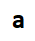
\includegraphics[height=.6cm]{figs/a.png}}
   \put(-330,105){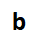
\includegraphics[height=.6cm]{figs/b.png}}
 \end{picture}
 \caption{Clustering of three droplets in a channel with a non-uniform inflow. \xx{(a) and (b) show the top (upper panel) and side (lower panel) view of the droplet positions under two initial conditions at different times.} The framed boxes depicts the actual computational domain \xx{(see Fig.\ \ref{fig: non-uniform sketch})}, in comparison to the Poiseuille channel in Fig.\ \ref{fig: poi results}. The color contours illustrate the velocity magnitude in two planes orthogonal to the viewing direction, \xx{where the color legend is the same as in Fig.\ \ref{fig: non-uniform sketch}}.}
 \label{fig: non-uniform}
\end{figure}

Figs.\ \ref{fig: non-uniform} and \ref{fig: non-uniform 4} demonstrate four representative cases of the self-assembly of three and four droplets, respectively, within a distance of $\sim 10D$ from their initial release. Specifically, the droplets in Fig.\ \ref{fig: non-uniform}(a) are initialized with $\theta_{open}=120$ deg.\ and $\theta_{dirc}=90$ deg. According to Fig.\ \ref{fig: poi results}b, this triplet would become a chain in the Poiseuille flow. Here, due to the rapid expansion of the flow immediately after the inlet, the trailing droplet undergoes a upward motion to the high velocity region; and if the velocity gained during this sprint is large enough, as in Fig.\ \ref{fig: non-uniform}(a), the droplets will soon form a triangle; otherwise, the cluster will at least form a V-shape pointing upstream, as shown in the example of Fig.\ \ref{fig: non-uniform}(b). In the latter cases, the final shape of the cluster can be estimated by its orientation relative to the flow (i.e.\ $\theta_{open}$ and $\theta_{dirc}$). Instead of simulating a full evolution of the clustering process (which may require a very large simulation domain and long time), one can simply read the last $(\theta_{open},\theta_{dirc})$ in the phase diagram of Fig.\ \ref{fig: poi results}(b). In the case discussed above (Fig.\ \ref{fig: non-uniform}(b)), we verified that a triangular cluster is eventually obtained (see ESI Video 2).

\begin{figure}[t]
 \centering
 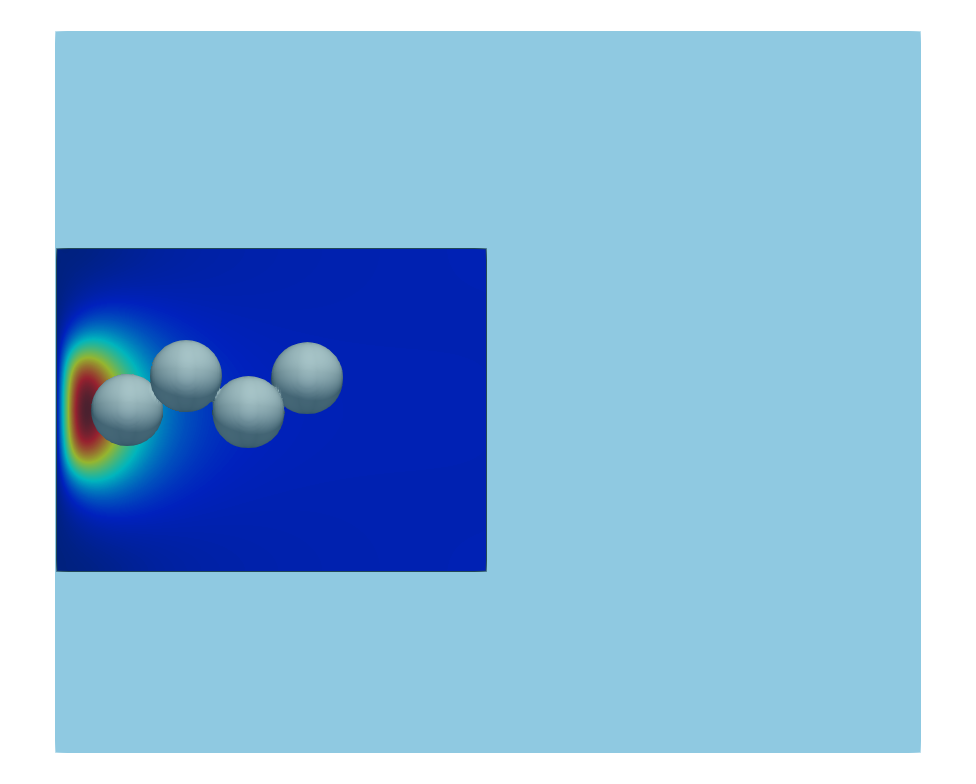
\includegraphics[width=.3\columnwidth]{figs/bd5-top-0.png}
 \includegraphics[width=.3\columnwidth]{figs/bd5-top-120k.png}
 \includegraphics[width=.3\columnwidth]{figs/bd5-top-250k.png}
 \includegraphics[width=.3\columnwidth]{figs/bd5-side-0-no.png}
 \includegraphics[width=.3\columnwidth]{figs/bd5-side-120k.png}
 \includegraphics[width=.3\columnwidth]{figs/bd5-side-250k.png}
 \includegraphics[width=.75\columnwidth]{figs/time_arrow.pdf}
 \includegraphics[width=.3\columnwidth]{figs/bd8-top-0.png}
 \includegraphics[width=.3\columnwidth]{figs/bd8-top-150k.png}
 \includegraphics[width=.3\columnwidth]{figs/bd8-top-450k.png}
 \includegraphics[width=.3\columnwidth]{figs/bd8-side-0.png}
 \includegraphics[width=.3\columnwidth]{figs/bd8-side-150k.png}
 \includegraphics[width=.3\columnwidth]{figs/bd8-side-450k.png}
 \begin{picture}(0,0)
   \put(-330,240){\includegraphics[height=.6cm]{figs/a.png}}
   \put(-330,105){\includegraphics[height=.6cm]{figs/b.png}}
 \end{picture}
 \caption{Clustering of four droplets in a channel with a non-uniform inflow. The organization of the plots is similar to Fig.\ \ref{fig: non-uniform}.}
 \label{fig: non-uniform 4}
\end{figure}

Similar observations are made for four droplets, for which we show two examples of clustering into diamond shapes in Fig.\ \ref{fig: non-uniform 4}. Here, the initial conditions are similar to those in Fig.\ \ref{fig: non-uniform}, only a fourth droplet is appended to the droplet string at a slightly lower vertical position (due to gravity). Note that the vertical coordinates of the droplets as they move downstream are in opposite orders (cf.\ the middle panels of Fig.\ \ref{fig: poi results}a). Consequently, the trailing droplets travel faster than the frontal ones, leading to the rapid closure of the cluster into more compact shapes.

The above examples clearly illustrate the direct effect of the non-uniform inflow. If properly matched with the initial droplet configuration, the droplets can form a compact structure within a much shorter distance than by the long-range dipolar interaction. And if the near-field depletion force is strong enough, the obtained compact cluster will stay bound further downstream. On the other hand, if the initial non-uniform inflow fails to bring the droplets sufficiently close within its range of influence, i.e. before viscous diffusion smoothens the initial velocity gradients (typically $\sim 10D$), the shear-induced cross-stream migration can break the clustering of the droplets, eventually leading to chain-like structures. This inflow effect, often neglected in theoretical models \citep{Shen_2016AS}, is what we propose to be the key reason for the accelerated droplet assembly.

Finally, we remark that the simulated inlet configuration is only one simplified version of the experimental microfluidic channel. To fully reproduce the condition in the actual setup is unrealistic due to the size contrast of the different inlets; however, it is perhaps also unnecessary as the qualitative features of the clustering do not depend on the fine details at the device level. Depending on the governing parameters and the specific operating conditions, it is possible to optimize the geometry of the microfluidic device to achieve higher throughputs of compact droplet clusters at the outlet; \xx{however, in practice, tuning of the geometry and inflow conditions may still involve trial and error, since the final self-assembly results from the combination of all $3D$ effects with no simple parametric dependence. This is possibly the bottleneck of upscaling the current microfluidic strategy to directly create large photonic crystals.}


\section{Summary and outlook}
\label{sec:summary}

Motivated by the recent experiment of flow-assisted droplet assembly \citep{Shen_2016AS} and its potential application for photonic material synthesis, we present a numerical study of finite numbers of non-Brownian droplets in a $3D$ microfluidic channel. The newly developed numerical methodology \citep{ICLS} allows for direct simulations of the two-fluid Navier-Stokes equations, and can account for the short-range attractive depletion force between the drops in a sharp fashion.

Under this framework, we considered three types of flows with increasing complexity: quiescent, confined simple shear, and pressure-driven channel flows. The case of quiescent flows allows us to disentangle the effect of the depletion force from that of the flow. The simulation of two to three droplets shows that the approaching time is inversely proportional to the osmotic number $\Pi$, a ratio between the surfactant-induced osmotic pressure and the Laplace pressure. We further assembled four to ten droplets using an arbitrary enumeration of the corresponding sphere packing. Without any external driving motion or noise, the obtained structure is purely determined by the closest neighbors in the initial state. This seemingly obvious result lays the basis for our subsequent reasoning.

As we place a droplet pair in the confined simple shear flow, the geometric obstruction combined with the depletion force results in a single steady configuration within the shear plane. The specific value of the alignment angle depends on the level of confinement and the shear rate; for nearly spherical drops between moving plates separated by $L_z/D =1.5$, we find the stable polar angle of the pair to be $\theta_\infty \approx 79$ deg. This alignment arises from the bifurcation of the relative trajectories of two droplets constrained by short-range attractive depletion forces. We expect the phenomenon to persist also for more than two drops, at least in the initial state where pairwise interaction dominates.

The dynamics of droplet clusters in the channel flow depends strongly on the homogeneity of the velocity profile. Using the reference Poiseuille flow, we find that the chain-like structure is far more favorable than the triangular cluster despite the latter is mechanically more stable. This is in contrast to $q2D$ systems where dipolar interactions provide the tangential motion destabilizing the droplet string. When the channel height is larger than the droplet diameter, as it is the case here, the dipolar flow becomes insignificant and the shear-induced cross-stream migration is a genuine $3D$ effect.

To fully understand the fast self-assembly observed in the experiment \citep{Shen_2016AS}, we also simulated three and four droplets near a step-emulsifier that is much smaller than the bulk channel. Under suitable initial conditions, the triplet/quadruplet indeed forms a more compact cluster from a chain. The nearly reversed inter-droplet motions comparing to the Poiseuille case clearly highlight the effect of the inhomogeneous flow. For practical microfluidic devices aiming for large throughputs, geometric optimization and fine tuning of the flow condition appear to be the key.

The above depicts the complete physical picture of depletion/hydrodynamic interactions of few non-Brownian droplets in a $3D$ microfluidic channel. \xx{Correctly identifying these mechanisms may help experimentalists design microfluidic chips not only for the fabrication of photonic metamaterials, but also other functionalities in general. We note that, although it remains a challenge to directly produce large, defect-free photonic crystals (typically of diamond-like structures) using the current microfluidic setup, alternative strategies have been recently proposed to \textit{indirectly} assembly droplet lattices composed of smaller clusters \citep{Konstantin}, or creating hyperuniform droplet ensembles using a similar microfluidic device \citep{Sal03,Joshua_2017PRL}. The latter is an active on-going research area, and we hope our findings provide additional guidelines to rationalize the design procedure of these miniature devices.}

\section*{Acknowledgments}

The work is supported by the Microflusa project. This effort receives funding from the European Union Horizon 2020 research and innovation programme under Grant Agreement No.\ 664823.
We thank Joshua Ricouvier and Bingqing Shen for providing the experimental details. Z.G.\ also thanks Mehdi Niazi, Alexander Leshansky, \AA smund Ervik, Zorana Zeravcic, and Tsvi Tlusty for helpful discussions.


\section*{Appendix}
\renewcommand\thesubsection{\Alph{subsection}} % redefine subsection labels (A,B,C...)

\subsection{Numerical setup} \label{app:numerics}

The simulations are performed in rectangular Cartesian domains with periodic and/or inflow-outflow boundary conditions in two directions and wall boundary condition (i.e.\ no slip/no penetration) in the third direction. The streamwise and spanwise dimensions of the computational box are at least three times bigger than the initial diameter of the droplet to prevent possible long-range interactions caused by the image droplet. The droplets are resolved by 32 grid points per diameter (i.e.\ $\Delta x=1/32$) to ensure that the interface curvature and the pressure jump are accurately computed, see \cite{ICLS} for detailed verification.

As mentioned earlier, the numerical values of $Re$ and $Ca$ are artificially increased to facilitate faster simulations over a larger parameter space. Specifically, we set $Re=10$, $Ca=0.005$ in Secs.\ \ref{sec:quiescent} and \ref{sec:poi}; $Re=1$, $Ca=0.0025$ in Sec.\ \ref{sec:shear}; and $Re=0.1$, $Ca=0.025$ in Sec.\ \ref{sec:non-uniform}. $Fr$ is effectively $\infty$ by setting the density ratio equal to unity in all cases except in Sec.\ \ref{sec:non-uniform}, where it is 0.025. The viscosity ratio is always 1. 

In Sec.\ \ref{sec:quiescent}, the suspending fluid has no underlying velocity, so the actual droplet Reynolds number should be rescaled by the ratio of the average approaching speed and the mean velocity of the channel \footnote{We keep the same definition of the Reynolds number due to bookkeeping reasons in the numerical code.}. In the case of two droplets, this factor is $1/64$ as one droplet moves the distance of $\Delta x$ within $t=2$, as comparing to a displacement of 2 within $t=2$. The rescaled Reynolds is then $Re_r \approx 0.16$.

\begin{figure}[t]
 \centering
 \includegraphics[width=.75\columnwidth]{figs/steady_angle1.pdf}
 \caption{Stable polar angle of two droplets in a shear-driven channel at different Reynolds numbers and confinement, cf.\ Sec.\ \ref{sec:shear}. \xx{The dashed line corresponds to $\theta_\infty=79$ deg.}}
 \label{fig: verify Re}
\end{figure}

In Sec.\ \ref{sec:shear}, we reduce $Re$ to 1 as the flow is shear-driven, thus the fluid inertia is expected to play a role. Testing various $Re$, as shown in Fig.\ \ref{fig: verify Re}, we observe that the stable polar angle approaches the same value for $Re \leqslant 1$ under the confinement of $L_z/D =1.5$, justifying the use of $Re=1$. For $L_z/D =3$, however, $Re<1$ must be used to obtain the true closed orbit of the two bounding pair (i.e.\ the obtained $\theta_\infty$ in that case is an artifact of the inertia).

In Sec.\ \ref{sec:poi}, we increase $Re$ to 10 as the cross-stream migration in Poiseuille flow is a fairly robust phenomenon, only weakly dependent on the Reynolds number in the sense that a lower $Re$ imposes a longer time scale. Since we are interested in the final shape of the droplet cluster - a qualitative result rather than the detail dynamics - $Re=10$ is used to speed up the simulations (the computational time step is roughly inversely proportional to $Re$).

Finally, in Sec.\ \ref{sec:non-uniform} where the entry region of the microfluidic channel is considered, we set the lowest Reynolds number to mimic the actual flow environment. Here, the capillary number is amplified to 0.025, larger than in the previous cases but still well within the low capillary limit. As a visual proof, the droplets shown in Fig.\ \ref{fig: non-uniform} all remain nearly spherical during the convection. Further reducing $Ca$ shall have no effect but refine the sphericity of the drops.


\subsection{Confinement-mediated interaction} \label{app:trajectory}

For unbounded simple shear flows, we know that a pair of spherical particles/droplets can undergo either closed orbits or open-and-symmetric trajectories \citep{batchelor_green_1972,Zinchenko1984}. With moderate confinements, swapping trajectories are also possible \citep{zurita-gotor_2007}. In Sec.\ \ref{sec:shear}, we show that strong geometric confinements combined with an attractive depletion force lead to pair alignments in the vorticity plane; particularly, the obtained stable polar angle is $\theta_\infty=79$ deg.\ for $L_z/D=1.5$. Below, we provide further evidence to support the symmetry-breaking argument and give a qualitative explanation of the observed $\theta_\infty$.

\begin{figure}[t]
 \centering
 \includegraphics[width=.85\columnwidth]{figs/traj.pdf}
 \caption{Relative trajectories of the second sphere in the vorticity plane of the simple-shear channel under confinement $L_z/D=1.5$. The pair is not constrained by any depletion force. The shaded region denotes locations inaccessible to the second droplet if it is perfectly spherical. Overlap of the trajectories with the shades is a result of the small droplet deformation. The red dot corresponds to the polar angle of 79 deg, c.f.\ Fig.\ \ref{fig: shell}.}
 \label{fig: traj}
\end{figure}

In Fig.\ \ref{fig: verify Re}, we obtain non-converging values of $\theta_\infty$ at $L_z/D=3$. Under this confinement, the binding droplets in the low-Reynolds-number limit exhibit cyclic motions as if they are unconfined (see ESI Video 3). Clearly, the center-to-center depletion force does not play any role since the hydrodynamic stresses already keep the droplet together; the droplets deform slightly, but are essentially spherical. As we double the confinement, i.e.\ reducing $L_z/D$ by half, Fig.\ \ref{fig: traj} illustrates the relative trajectories in the absence of depletion forces (see also ESI Video 4,5). Here, only a quadrant of the plane in the vicinity of the first droplet is shown due to symmetry. Comparing to less confined conditions, the droplet pair displays only passing and swapping trajectories, while the Batchelor-Green type of closed orbit is completely suppressed (c.f.\ Fig.\ 3 in \citep{zurita-gotor_2007}). Arguably, such a result is obvious as the droplets cannot simply rotate in the same vorticity plane, whereas $3D$ rotations would violate either time-reversal or mirror symmetry. \footnote{The symmetry argument, however, is only a necessary but not sufficient condition, since droplet sliding on the walls already invokes effects of the noise (otherwise two droplets stuck by the walls should be regarded as an admissible solution).} Regardless the reason, the results demonstrate that droplets cannot stay together indefinitely due solely to the hydrodynamic interactions. More importantly, plotting the position corresponding to the angle of 79 deg.\ (the red dot in Fig.\ \ref{fig: traj}) in the trajectory map clearly rationalizes the existence of a stable polar angle: the second droplet would travel in either direction above or below the saddle point; with a radial depletion force, only at $\theta_\infty=79$ deg.\ can it stay dynamically stable.



%--%\bigskip
%--%
%--%
%--%%%%%%%%%%%%%%%%%%%%%%%%%%%%%%%%%%%%%%%%%%%%%%%%%%%%%%%%
%--%\iffalse
%--%
%--%Adding notes to tables can be complicated.  Perhaps the easiest method is to generate these manually.\footnote[4]{Footnotes should appear here. These might include comments relevant to but not central to the matter under discussion, limited experimental and spectral data, and crystallographic data.}
%--%
%--%\begin{table*}
%--%\small
%--%  \caption{\ An example of a caption to accompany a table \textendash\ table captions do not end in a full point}
%--%  \label{tbl:example2}
%--%  \begin{tabular*}{\textwidth}{@{\extracolsep{\fill}}lllllll}
%--%    \hline
%--%    Header one & Header two & Header three & Header four & Header five & Header six  & Header seven\\
%--%    \hline
%--%    1 & 2 & 3 & 4 & 5 & 6  & 7\\
%--%    8 & 9 & 10 & 11 & 12 & 13 & 14 \\
%--%    15 & 16 & 17 & 18 & 19 & 20 & 21\\
%--%    \hline
%--%  \end{tabular*}
%--%\end{table*}
%--%
%--%\section{Equations}
%--%
%--%Equations can be typeset inline \textit{e.g.}\ $ y = mx + c$ or displayed with and without numbers:
%--%
%--% \[ A = \pi r^2 \]
%--%
%--%\begin{equation}
%--%  \frac{\gamma}{\epsilon x} r^2 = 2r
%--%\end{equation}
%--%
%--%You can also put lists into the text. You can have bulleted or numbered lists of almost any kind. 
%--%The \texttt{mhchem} package can also be used so that formulae are easy to input: \texttt{\textbackslash ce\{H2SO4\}} gives \ce{H2SO4}. 
%--%
%--%For footnotes in the main text of the article please number the footnotes to avoid duplicate symbols. \textit{e.g.}\ \texttt{\textbackslash footnote[num]\{your text\}}. The corresponding author $\ast$ counts as footnote 1, ESI as footnote 2, \textit{e.g.}\ if there is no ESI, please start at [num]=[2], if ESI is cited in the title please start at [num]=[3] \textit{etc.} Please also cite the ESI within the main body of the text using \dag.
%--%
%--%\fi
%--%
%--%%%%END OF MAIN TEXT%%%
%--%
%--%%The \balance command can be used to balance the columns on the final page if desired. It should be placed anywhere within the first column of the last page.
%--%
%--%\balance
%--%
%--%%If notes are included in your references you can change the title from 'References' to 'Notes and references' using the following command:
%--%%\renewcommand\refname{Notes and references}
%--%
%--%%%%REFERENCES%%%
%--%\bibliography{main} %You need to replace "rsc" on this line with the name of your .bib file
%--%\bibliographystyle{rsc} %the RSC's .bst file
%--%
%--%
%--%\end{document}
